\documentclass[10pt,twocolumn,letterpaper]{article}

\usepackage{cvpr}
\usepackage{times}
\usepackage{epsfig}
\usepackage{graphicx}
\usepackage{amsmath,amssymb,bm}

% Include other packages here, before hyperref.

% If you comment hyperref and then uncomment it, you should delete
% egpaper.aux before re-running latex.  (Or just hit 'q' on the first latex
% run, let it finish, and you should be clear).
\usepackage[pagebackref=false,breaklinks=true,letterpaper=true,colorlinks,bookmarks=false]{hyperref}
\hyphenpenalty=1500
\cvprfinalcopy % *** Uncomment this line for the final submission

\def\cvprPaperID{399} % *** Enter the CVPR Paper ID here
\def\httilde{\mbox{\tt\raisebox{-.5ex}{\symbol{126}}}}

% Pages are numbered in submission mode, and unnumbered in camera-ready
\ifcvprfinal\pagestyle{empty}\fi


\newcommand{\datasetName}{CompCars}

\begin{document}

%%%%%%%%% TITLE
\title{A Large-Scale Car Dataset for Fine-Grained Categorization and Verification}

\author{Linjie Yang$^{1}$~~~~~~~~~~~~Ping Luo$^{2,1}$~~~~~~~~~~~~Chen Change Loy$^{1,2}$~~~~~~~~~~~~Xiaoou Tang$^{1,2}$\\
$^1$Department of Information Engineering, The Chinese University of Hong Kong\\
$^2$Shenzhen Key Lab of CVPR, Shenzhen Institutes of Advanced Technology, \\
Chinese Academy of Sciences, Shenzhen, China\\
{\tt\small \{yl012,pluo,ccloy,xtang\}@ie.cuhk.edu.hk}
}

\maketitle
%\thispagestyle{empty}

%%%%%%%%% ABSTRACT
\begin{abstract}
This paper aims to highlight vision related tasks centered around ``car'', which has been largely neglected by vision community in comparison to other objects.
%
We show that there are still many interesting car-related problems and applications, which are not yet well explored and researched.
%
To facilitate future car-related research, in this paper we present our on-going effort in collecting a large-scale dataset, ``CompCars'', that covers not only different car views, but also their different internal and external parts, and rich attributes. Importantly, the dataset is constructed with a cross-modality nature, containing a surveillance-nature set and a web-nature set. We further demonstrate a few important applications exploiting the dataset, namely car model classification, car model verification, and attribute prediction. We also discuss specific challenges of the car-related problems and other potential applications that worth further investigations.
%
The latest dataset can be downloaded at \url{http://mmlab.ie.cuhk.edu.hk/datasets/comp_cars/index.html}

** Update: This technical report serves as an extension to our earlier work~\cite{yang2015large} published in CVPR 2015. The experiments shown in Sec.~\ref{sec:updated} gain better performance on all three tasks, \ie~car model classification, attribute prediction, and car model verification, thanks to more training data and better network structures. The experimental results can serve as baselines in any later research works. The settings and the train/test splits are provided on the project page.


  %%The problem of car model analysis is of critical demand in the real world applications but attracts few attentions. Existing car model datasets are limited by their category number and data varieties, failing to meet the need for realistic applications. We organize a large scale image dataset containing 1751 different car models and 286,045 images from two scenarios, web-nature and surveillance-nature. With rich and interesting features such as model attributes and car parts, the dataset is ready to be utilized for enormous novel research topics. We conduct three sets of experiments: car model classification, car model verification, and attribute prediction. The experiment results prove the usefulness of our dataset and provide several insights into the related problems. We also conduct a cross-scenario experiment, using the web-nature data for training and surveillance-nature data for testing. The cross-scenario capability of our model reveals the potential of the dataset for realistic applications.

** Update 2: This update provides preliminary experiment results for fine-grained classification on the surveillance data of CompCars. The train/test splits are provided in the updated dataset. See details in Section~\ref{sec:surveillance}.
\end{abstract}

%%%%%%%%% BODY TEXT
\section{Introduction}

\begin{figure}[t]\centering
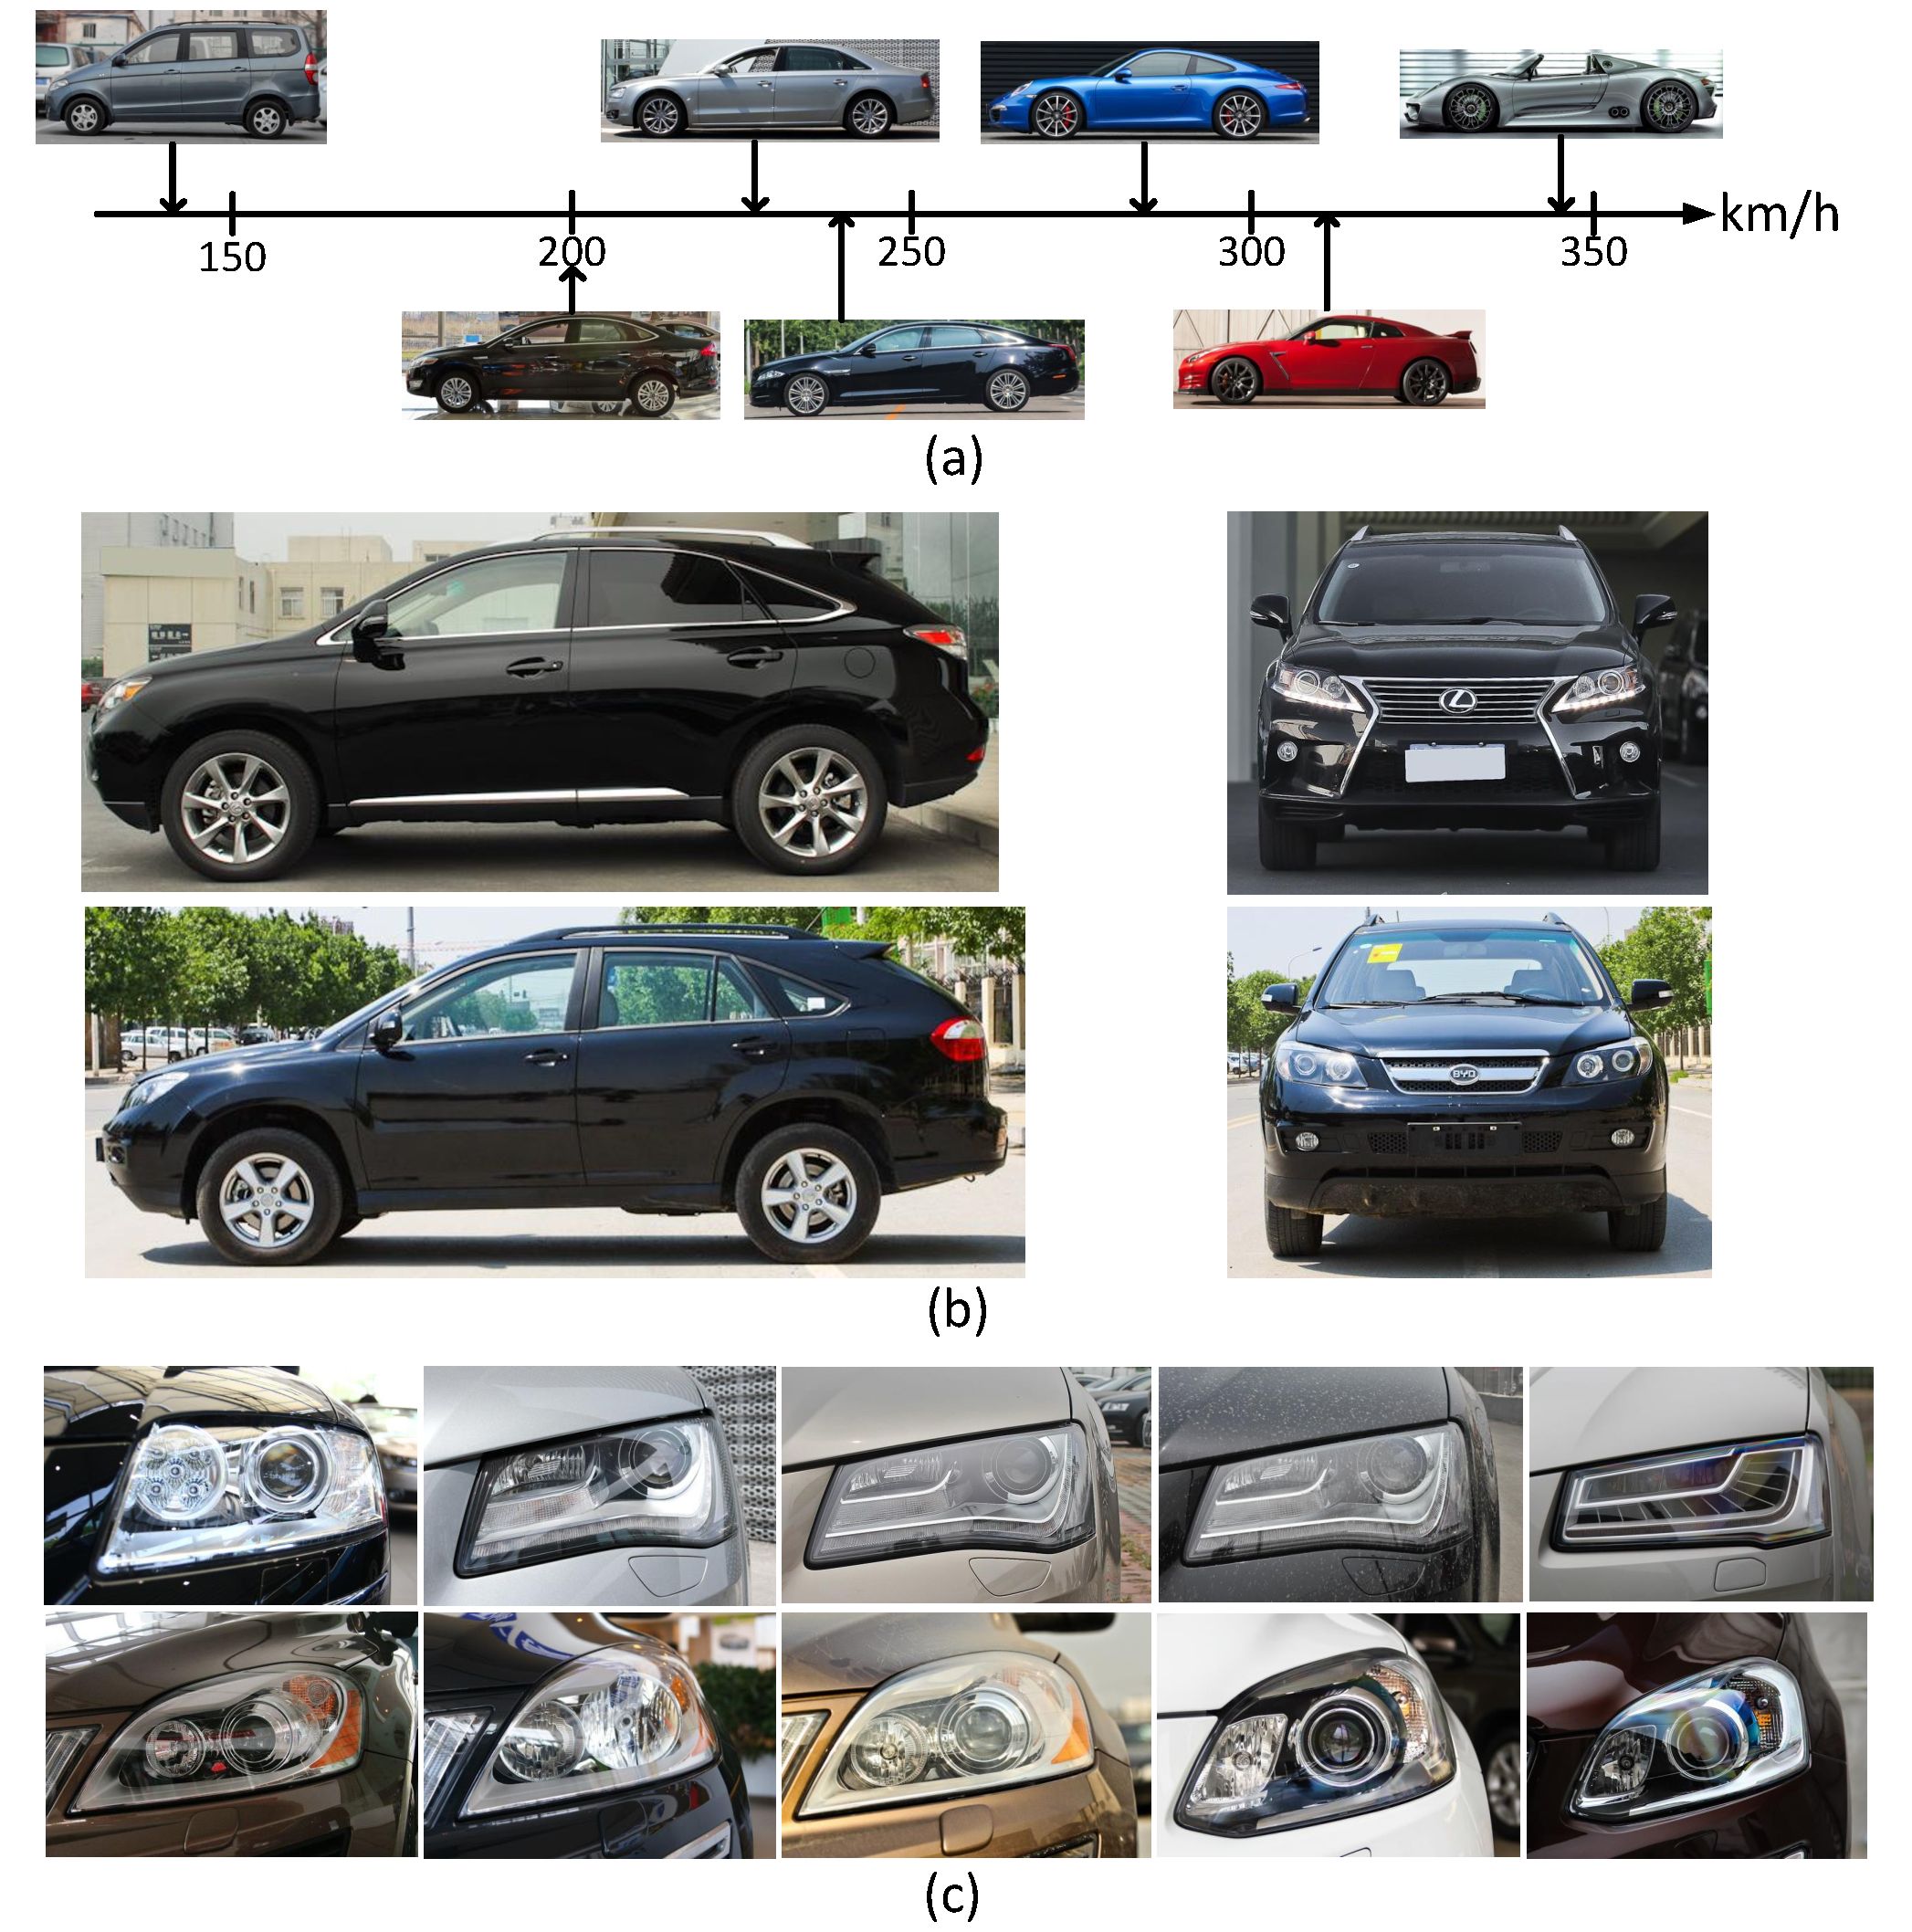
\includegraphics[width=1\linewidth]{interest.pdf}
\caption{(a) Can you predict the maximum speed of a car with only a photo? Get some cues from the examples. (b) The two SUV models are very similar in their side views, but are rather different in the front views. (c) The evolution of the headlights of two car models from 2006 to 2014 (left to right).}
\label{fig:interest}
\vspace{-4pt}
\end{figure}

Cars represent a revolution in mobility and convenience, bringing us the flexibility of moving from place to place. The societal benefits (and cost) are far-reaching.
%
Cars are now indispensable from our modern life as a vehicle for transportation.
%
In many places, the car is also viewed as a tool to help project someone's economic status, or reflects our economic stratification. In addition, the car has evolved into a subject of interest amongst many car enthusiasts in the world.
%
In general, the demand on car has shifted over the years to cover not only practicality and reliability, but also high comfort and design.
%
The enormous number of car designs and car model makes car a rich object class, which can potentially foster more sophisticated and robust computer vision models and algorithms.



%The year 1886 is regarded as the birth year of the modern car. Since then, humans are granted with the flexibility of moving from place to place.
%
%In many cities, a car is practically required to get and keep a job because of poor public transport system.
%
%Global automobile sales are expected to reach 88.6 million in 2015
%
%The worldwide automotive industry has been enjoying a period of relatively strong growth
%forecasting annualized sales in North America in the near term of a relatively robust 16 million cars









%Cars are ubiquitous in our daily life. People drive cars to work, on travel, or for racing. A car helps you get to places wherever you want to reach. But how much do you know about your car? How do you identify your car from the others? Which viewpoint helps you best to identify the model of a car? How does the appearance of cars evolve through the years? How does the shape of car change from lower-end to luxury?

%%Being familiar and mysterious, cars inspire our imaginations for a range of novel computer vision topics, such as car model recognition / verification, predicting attributes of an unknown car, and style analysis of cars. %%refer to Fig.1 for some tasks.
%%data specialties --> facilitate noval tasks --> innovate other fields in computer vision

%From computer vision perspective, cars are valuable subject to develop and test our algorithms.

Cars present several unique properties that other objects cannot offer, which provides more challenges and facilitates a range of novel research topics in object categorization.
%
Specifically, cars own large quantity of models that most other categories do not have, enabling a more challenging fine-grained task.
%
In addition, cars yield large appearance differences in their unconstrained poses, which demands viewpoint-aware analyses and algorithms (see Fig.~\ref{fig:interest}(b)).
%
Importantly, a unique hierarchy is presented for the car category, which is three levels from top to bottom: make, model, and released year. This structure indicates a direction to address the fine-grained task in a hierarchical way, which is only discussed by limited literature~\cite{Maji13}.
%
Apart from the categorization task, cars reveal a number of interesting computer vision problems.
%
Firstly, different designing styles are applied by different car manufacturers and in different years, which opens the door to fine-grained style analysis~\cite{Lee13style} and fine-grained part recognition (see Fig.~\ref{fig:interest}(c)).
%
Secondly, the car is an attractive topic for attribute prediction. In particular, cars have distinctive attributes such as car class, seating capacity, number of axles, maximum speed and displacement, which can be inferred from the appearance of the cars (see Fig.~\ref{fig:interest}(a)).
%
Lastly, in comparison to human face verification~\cite{Sun14}, car verification, which targets at verifying whether two cars belong to the same model, is an interesting and under-researched problem. The unconstrained viewpoints make car verification arguably more challenging than traditional face verification.


%%Indetifying cars are in surveillance. Face recognition~\cite{Chen12}~\cite{Sun14}~\cite{Taigman14} and person re-identification~\cite{Farenzena10}~\cite{Zhao13} designate at discovering the human identity in the surveillance cameras.

Automated car model analysis, particularly the fine-grained car categorization and verification, can be used for innumerable purposes in intelligent transportation system including regulation, description and indexing.
%
For instance, fine-grained car categorization can be exploited to inexpensively automate and expedite paying tolls from the lanes, based on different rates for different types of vehicles.
%
%Electronic toll collection (ETC) aims to eliminate the delay on toll roads by collecting tolls electronically.
%
In video surveillance applications, car verification from appearance helps tracking a car over a multiple camera network when car plate recognition fails.
%
In post-event investigation, similar cars can be retrieved from the database with car verification algorithms.
%
Car model analysis also bears significant value in the personal car consumption.
%
When people are planning to buy cars, they tend to observe cars in the street. Think of a mobile application, which can instantly show a user the detailed information of a car once a car photo is taken. Such an application will provide great convenience when people want to know the information of an unrecognized car. Other applications such as predicting popularity based on the appearance of a car, and recommending cars with similar styles can be beneficial both for manufacturers and consumers.
%%add examples: report, etc.

%analyse market segment, microcar, compact car, luxury car,  multi-purpose vehicle  MPV, sport utility vehicles SUV


%Global online car sales are expected to increase eightfold between 2011 and 2025 to almost \$4.5bn,  to more online-focused retailing, as more and more buyers in markets such as India, Brazil and China use manufacturer websites and view online advertising in deciding on which model to buy.



%%not well solve
Despite the huge research and practical interests, car model analysis only attracts few attentions in the computer vision community.
%
We believe the lack of high quality datasets greatly limits the exploration of the community in this domain.
%
To this end, we collect and organize a large-scale and comprehensive image database called ``Comprehensive Cars'', with ``CompCars'' being short.
%
The ``CompCars'' dataset is much larger in scale and diversity compared with the current car image datasets, containing $208,826$ images of $1,716$ car models from two scenarios: web-nature and surveillance-nature.
%
In addition, the dataset is carefully labelled with viewpoints and car parts, as well as rich attributes such as type of car, seat capacity, and door number.
%
%With more than XX times of the image numbers and more than 8 times of the subcategory numbers of the latest fine-grained car datasets~\cite{} \textbf{(give reference)}, and with rich attributes (\eg~viewpoints, car parts, type of car),
%
The new dataset dataset thus provides a comprehensive platform to validate the effectiveness of a wide range of computer vision algorithms. It is also ready to be utilized for realistic applications and enormous novel research topics. Moreover, the multi-scenario nature enables the use of the dataset for cross modality research. The detailed description of \datasetName{} is provided in Section~\ref{sec:dataset}.


To validate the usefulness of the dataset and to encourage the community to explore for more novel research topics, we demonstrate several interesting applications with the dataset, including car model classification and verification based on convolutional neural network (CNN)~\cite{Lecun1989}. Another interesting task is to predict attributes from novel car models (see details in Section~\ref{sec:attr}). The experiments reveal several challenges specific to the car-related problems.
%
We conclude our analyses with a discussion in Section~\ref{sec:discussion}.
%We believe this dataset will provide a bridge between the latest research on computer vision and part of the urgent demand in our society.



\section{Related Work}

%Car model classification has been a popular topic recent years but the works are mostly restricted to a small number of car model categories.

Most previous car model research focuses on car model classification. Zhang \etal~\cite{Zhang12} propose an evolutionary computing framework to fit a wireframe model to the car on an image. Then the wireframe model is employed for car model recognition.
%
Hsiao \etal~\cite{Hsiao14} construct 3D space curves using 2D training images, then match the 3D curves to 2D image curves using a 3D view-based alignment technique. The car model is finally determined with the alignment result.
%
Lin \etal~\cite{Lin14} optimize 3D model fitting and fine-grained classification jointly. All these works are restricted to a small number of car models. Recently, Krause et al.~\cite{Krause13} propose to extract 3D car representation for classifying 196 car models. The experiment is the largest scale that we are aware of.
%
Car model classification is a fine-grained categorization task.
%
In contrast to general object classification, fine-grained categorization targets at recognizing the subcategories in one object class. Following this line of research, many studies have proposed different datasets on a variety of categories: birds~\cite{CUB_200}, dogs~\cite{Liu12dog}, cars~\cite{Krause13}, flowers~\cite{Nilsback08}, etc. But all these datasets are limited by their scales and subcategory numbers.
%How recognizing a bird can benefit us aside from the bird amateurs?

To our knowledge, there is no previous attempt on the car model verification task.
%
Closely related to car model verification, face verification has been a popular topic~\cite{LFWTech,Kumar09,Sun14,ZhuNIPS2014}. The recent deep learning based algorithms~\cite{Sun14} first train a deep neural network on human identity classification, then train a verification model with the feature extracted from the deep neural network. Joint Bayesian~\cite{Chen12} is a widely-used verification model that models two faces jointly with an appropriate prior on the face representation. We adopt Joint Bayesian as a baseline model in car model verification.

%As a close related topic, face verification has attracted lots of attention in the literature. Car model verification is more challenging than face verification with the following facts. First, cars can be viewed from any viewpoint from a viewing sphere, resulting in completely different appearance, while most face images are in the front or near front view. Second, faces can be aligned with the keypoints which are shared by all human faces, while cars hardly share any keypoints even in the same viewpoint. Third, most cars are with spectacular surfaces, which increases their appearance variations.

%%works on attr prediction
%Attributes are used to assist different tasks: object recognition~\cite{}, face verification~\cite{}, .
Attribute prediction of humans is a popular research topic in recent years~\cite{Bourdev11,DengMM2014,Kumar09,Zhang14}. However, a large portion of the labeled attributes in the current attribute datasets~\cite{DengMM2014}, such as \emph{long hair} and \emph{short pants} lack strict criteria, which causes annotation ambiguities~\cite{Bourdev11}. The attributes with ambiguities will potentially harm the effectiveness of evaluation on related datasets. In contrast, the attributes provided by \datasetName{} (\eg~maximum speed, door number, seat capacity) all have strict criteria since they are set by the car manufacturers. The dataset is thus advantageous over the current datasets in terms of the attributes validity.

%other car related research
Other car-related research includes detection~\cite{Sun06}, tracking~\cite{Matei11}~\cite{Xiang14}, joint detection and pose estimation~\cite{He14, Yang14}, and 3D parsing~\cite{Zia14}. Fine-grained car models are not explored in these studies. Previous research related to car parts includes car logo recognition~\cite{Psyllos10} and car style analysis based on mid-level features~\cite{Lee13style}.

Similar to \datasetName{}, the Cars dataset~\cite{Krause13} also targets at fine-grained tasks on the car category. Apart from the larger-scale database, our \datasetName{} dataset offers several significant benefits in comparison to the Cars dataset.
%
First, our dataset contains car images diversely distributed in all viewpoints (annotated by front, rear, side, front-side, and rear-side), while Cars dataset mostly consists of front-side car images. Second, our dataset contains aligned car part images, which can be utilized for many computer vision algorithms that demand precise alignment. Third, our dataset provides rich attribute annotations for each car model, which are absent in the Cars dataset.

\section{Properties of \datasetName{}}\label{sec:dataset}


The \datasetName{} dataset contains data from two scenarios, including images from \emph{web-nature} and \emph{surveillance-nature}.
%
The images of the web-nature are collected from car forums, public websites, and search engines.
%
The images of the surveillance-nature are collected by surveillance cameras. The data of these two scenarios are widely used in the real-world applications.
%
They open the door for cross-modality analysis of cars.
%
In particular, the web-nature data contains $163$ car makes with $1,716$ car models, covering most of the commercial car models in the recent ten years.
%
There are a total of $136,727$ images capturing the entire cars and $27,618$ images capturing the car parts, where most of them are labeled with attributes and viewpoints.
%
%We also labeled and organized interesting features such as car model attributes and viewpoints for the web-nature data.
The surveillance-nature data contains $44,481$ car images captured in the front view.
%
Each image in the surveillance-nature partition is annotated with bounding box, model, and color of the car.
%The labeling provides information of bounding box, car model, and car color.
Fig.~\ref{fig:sv_data} illustrates some examples of surveillance images, which are affected by large variations from lightings and haze.
%
Note that the data from the surveillance-nature are significantly different from the web-nature data in Fig.~\ref{fig:interest}, suggesting the great challenges in cross-scenario car analysis.
%
Overall, the \datasetName{} dataset offers four unique features in comparison to existing car image databases, namely car hierarchy, car attributes, viewpoints, and car parts.
%
%With this dataset, we conduct several cross-scenario experiments to demonstrate its potential in practical applications.

%Notice the appearance difference of the surveillance-nature images in Fig.~\ref{fig:sv_data} and the web-nature images in Fig.~\ref{fig:interest}.
%We conduct a cross-scenario experiment to illustrate the potential of our dataset for real applications in Section~\ref{sec:cls}. In the following, four interesting features of the web-nature data are introduced: hierarchy, attributes, viewpoint annotation, and car parts.
%The dataset is still keep expanding for extra car models, images, and interesting attributes. %%how to describe the validity of the labels: model, attributes


\begin{figure}[t]\centering
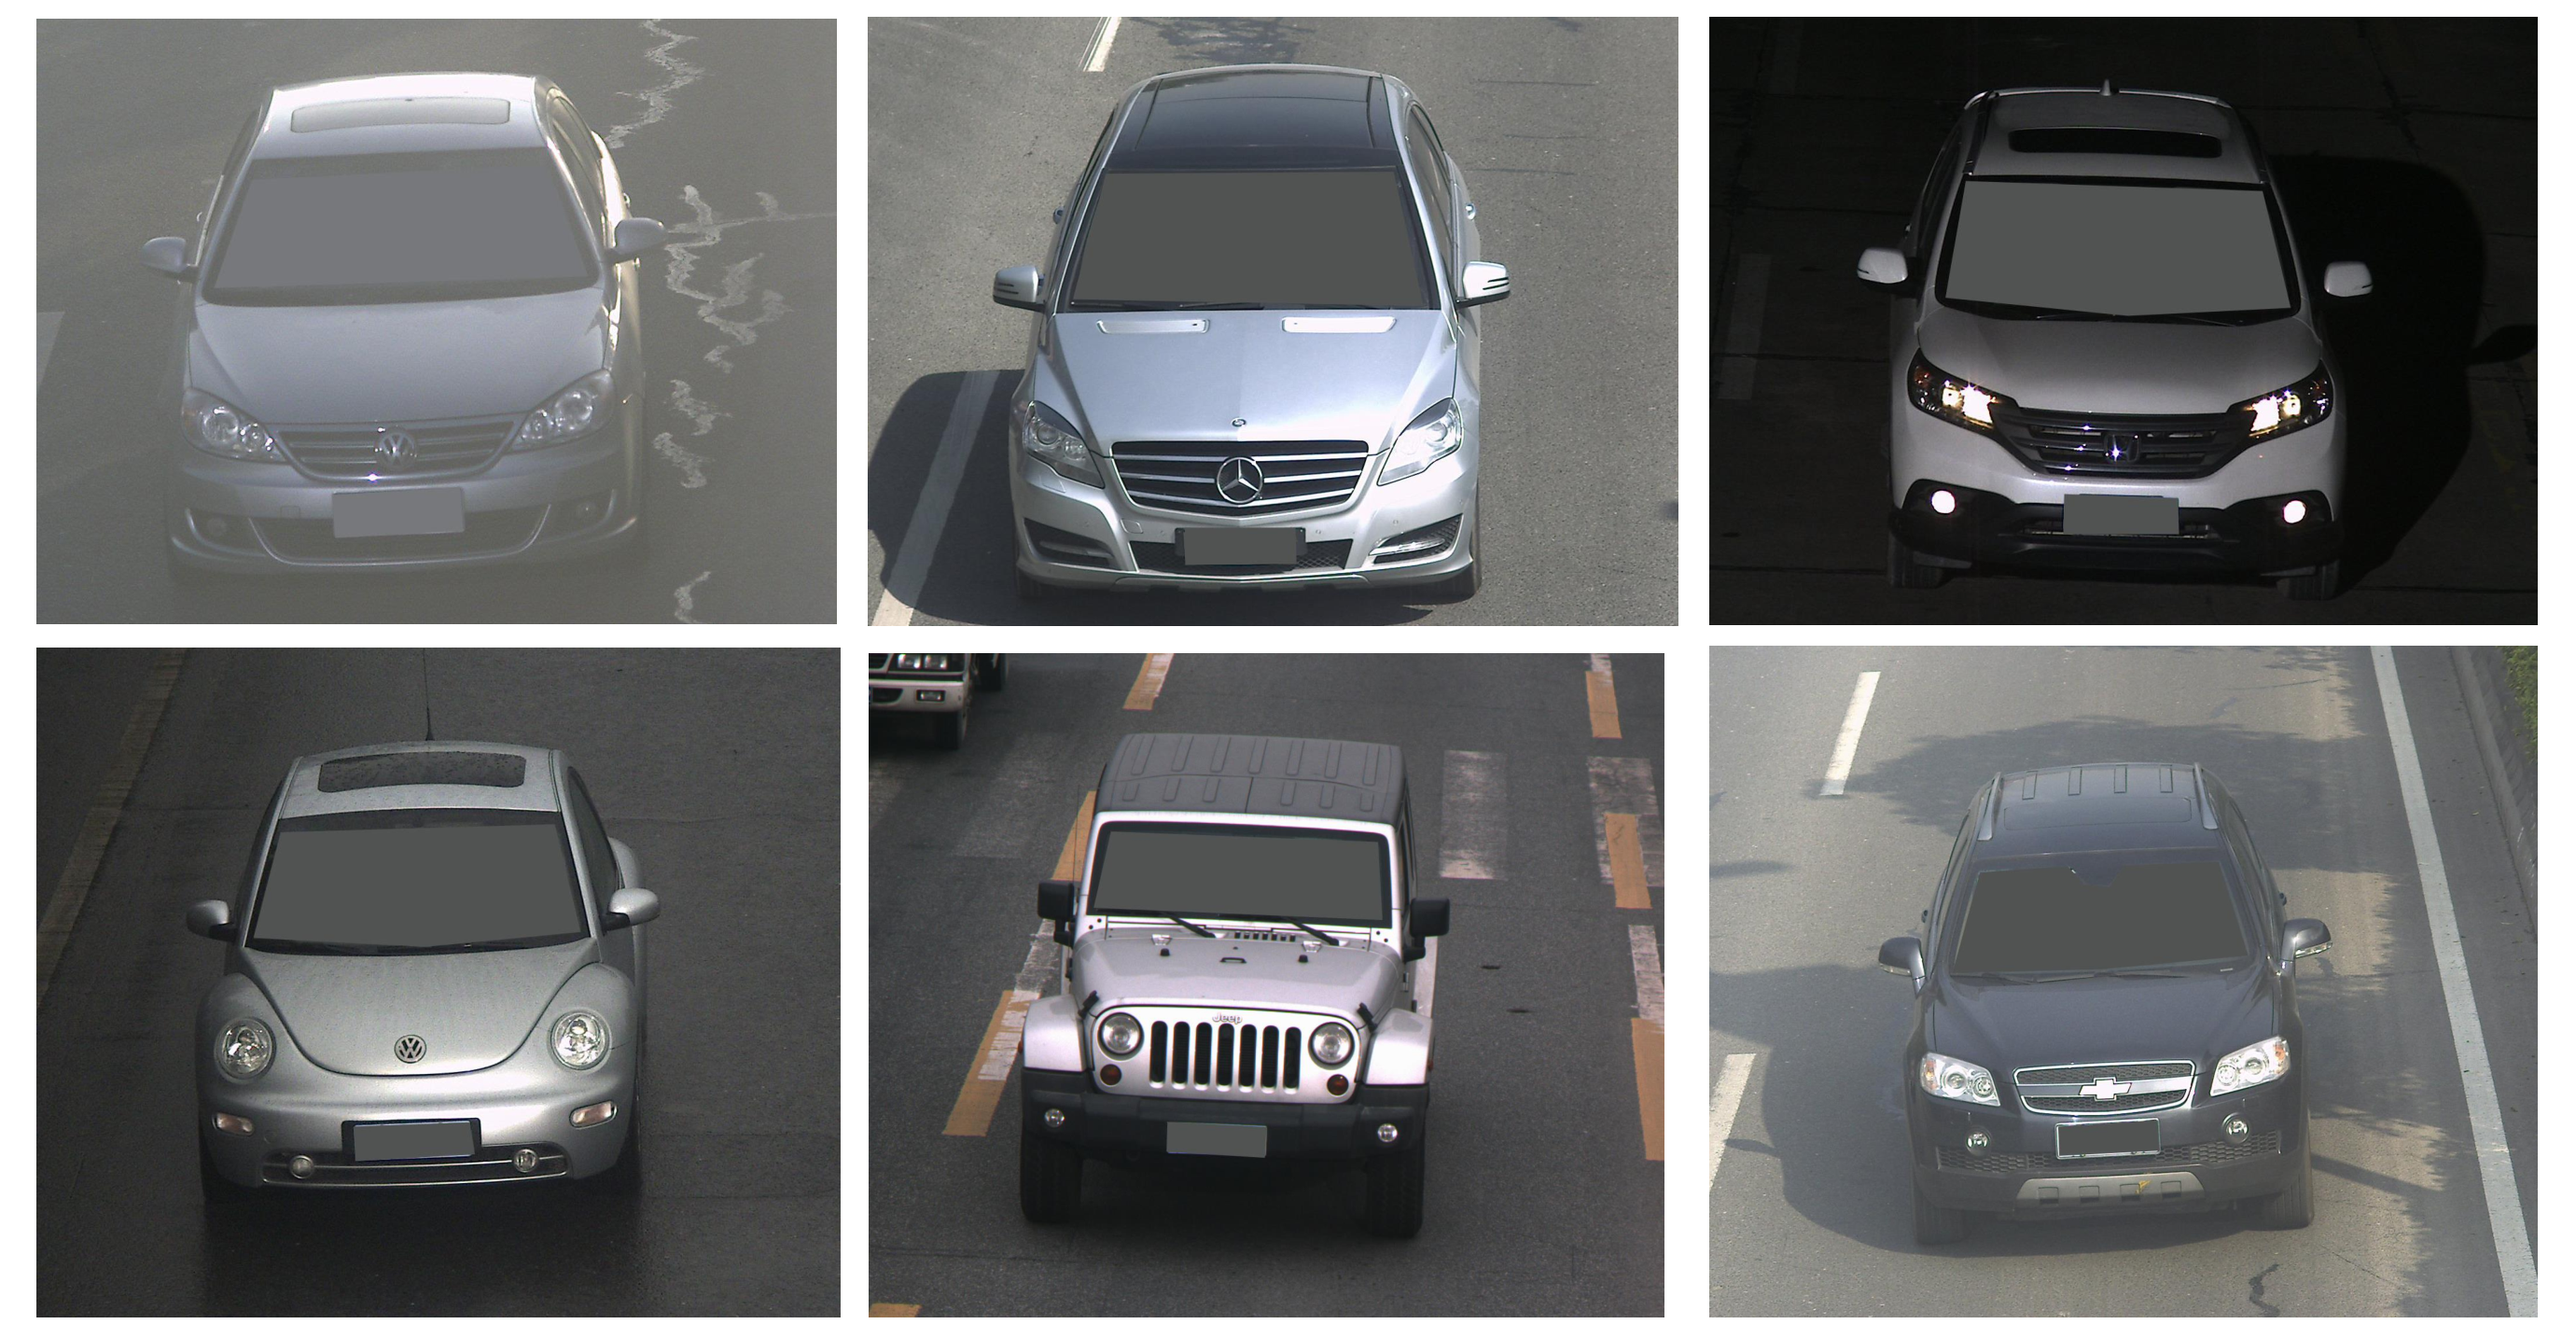
\includegraphics[width=0.9\linewidth]{sv_data.pdf}
\caption{Sample images of the surveillance-nature data. The images have large appearance variations due to the varying conditions of light, weather, traffic, etc.}
\label{fig:sv_data}
\vspace{-4pt}
\end{figure}

%\begin{figure}[t]\centering
%\includegraphics[width=1\linewidth]{similar.pdf}
%\caption{Front view of four similar car models of Volkswagen. The model names are Santana, Golf convertible, Golf estate, and Golf, respectively ((a)--(d)). It is hard even for a human to tell them apart.}
%\label{fig:similar}
%\end{figure}

\begin{figure}[t]\centering
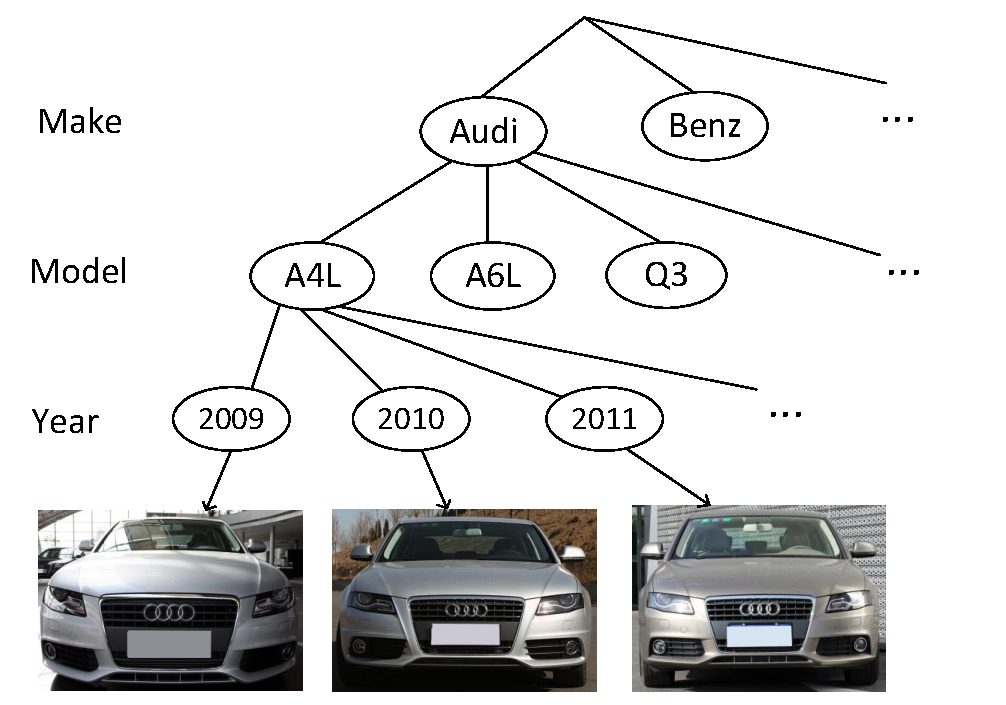
\includegraphics[width=0.8\linewidth]{tree.pdf}
\caption{The tree structure of car model hierarchy. Several car models of Audi A4L in different years are also displayed. }
\label{fig:tree}
\vspace{-4pt}
\end{figure}

\textbf{Car Hierarchy}
The car models can be organized into a large tree structure, consisting of three layers , namely car make, car model, and year of manufacture, from top to bottom as depicted in Fig.~\ref{fig:tree}.
%
The complexity is further compounded by the fact that each car model can be produced in different years, yielding subtle difference in their appearances. For instance, three versions of ``Audi A4L'' were produced between 2009 to 2011 respectively.

%. Levels of the tree are make, model, and released year from top to down. Each make has different models. And each model has different versions on different years, which have relatively. Fig.~\ref{fig:tree} illustrates the tree structure which also displays car models of Audi A4L in different years. In this work, we only focus on the classification on the model category level. Nevertheless, the dataset can be exploited to address more challenging problems such as recognizing the different versions from different years.

%The car models can be naturally organized with a tree structure. Levels of the tree are make, model, and released year from top to down. Each make has different models. And each model has different versions on different years, which have relatively subtle difference in appearance. Fig.~\ref{fig:tree} illustrates the tree structure which also displays car models of Audi A4L in different years. In this work, we only focus on the classification on the model category level. Nevertheless, the dataset can be exploited to address more challenging problems such as recognizing the different versions from different years.

%Different models of the same brand can also be similar in appearance. Fig.~\ref{fig:similar} illustrates the front view of several very similar car models of Volkswagen, which is hard even for a human to tell them apart.
%%brands, branch, model, model_year
%the model-year level categories have very subtle difference so we focus on classification based on the model level.
\begin{figure}[t]\centering
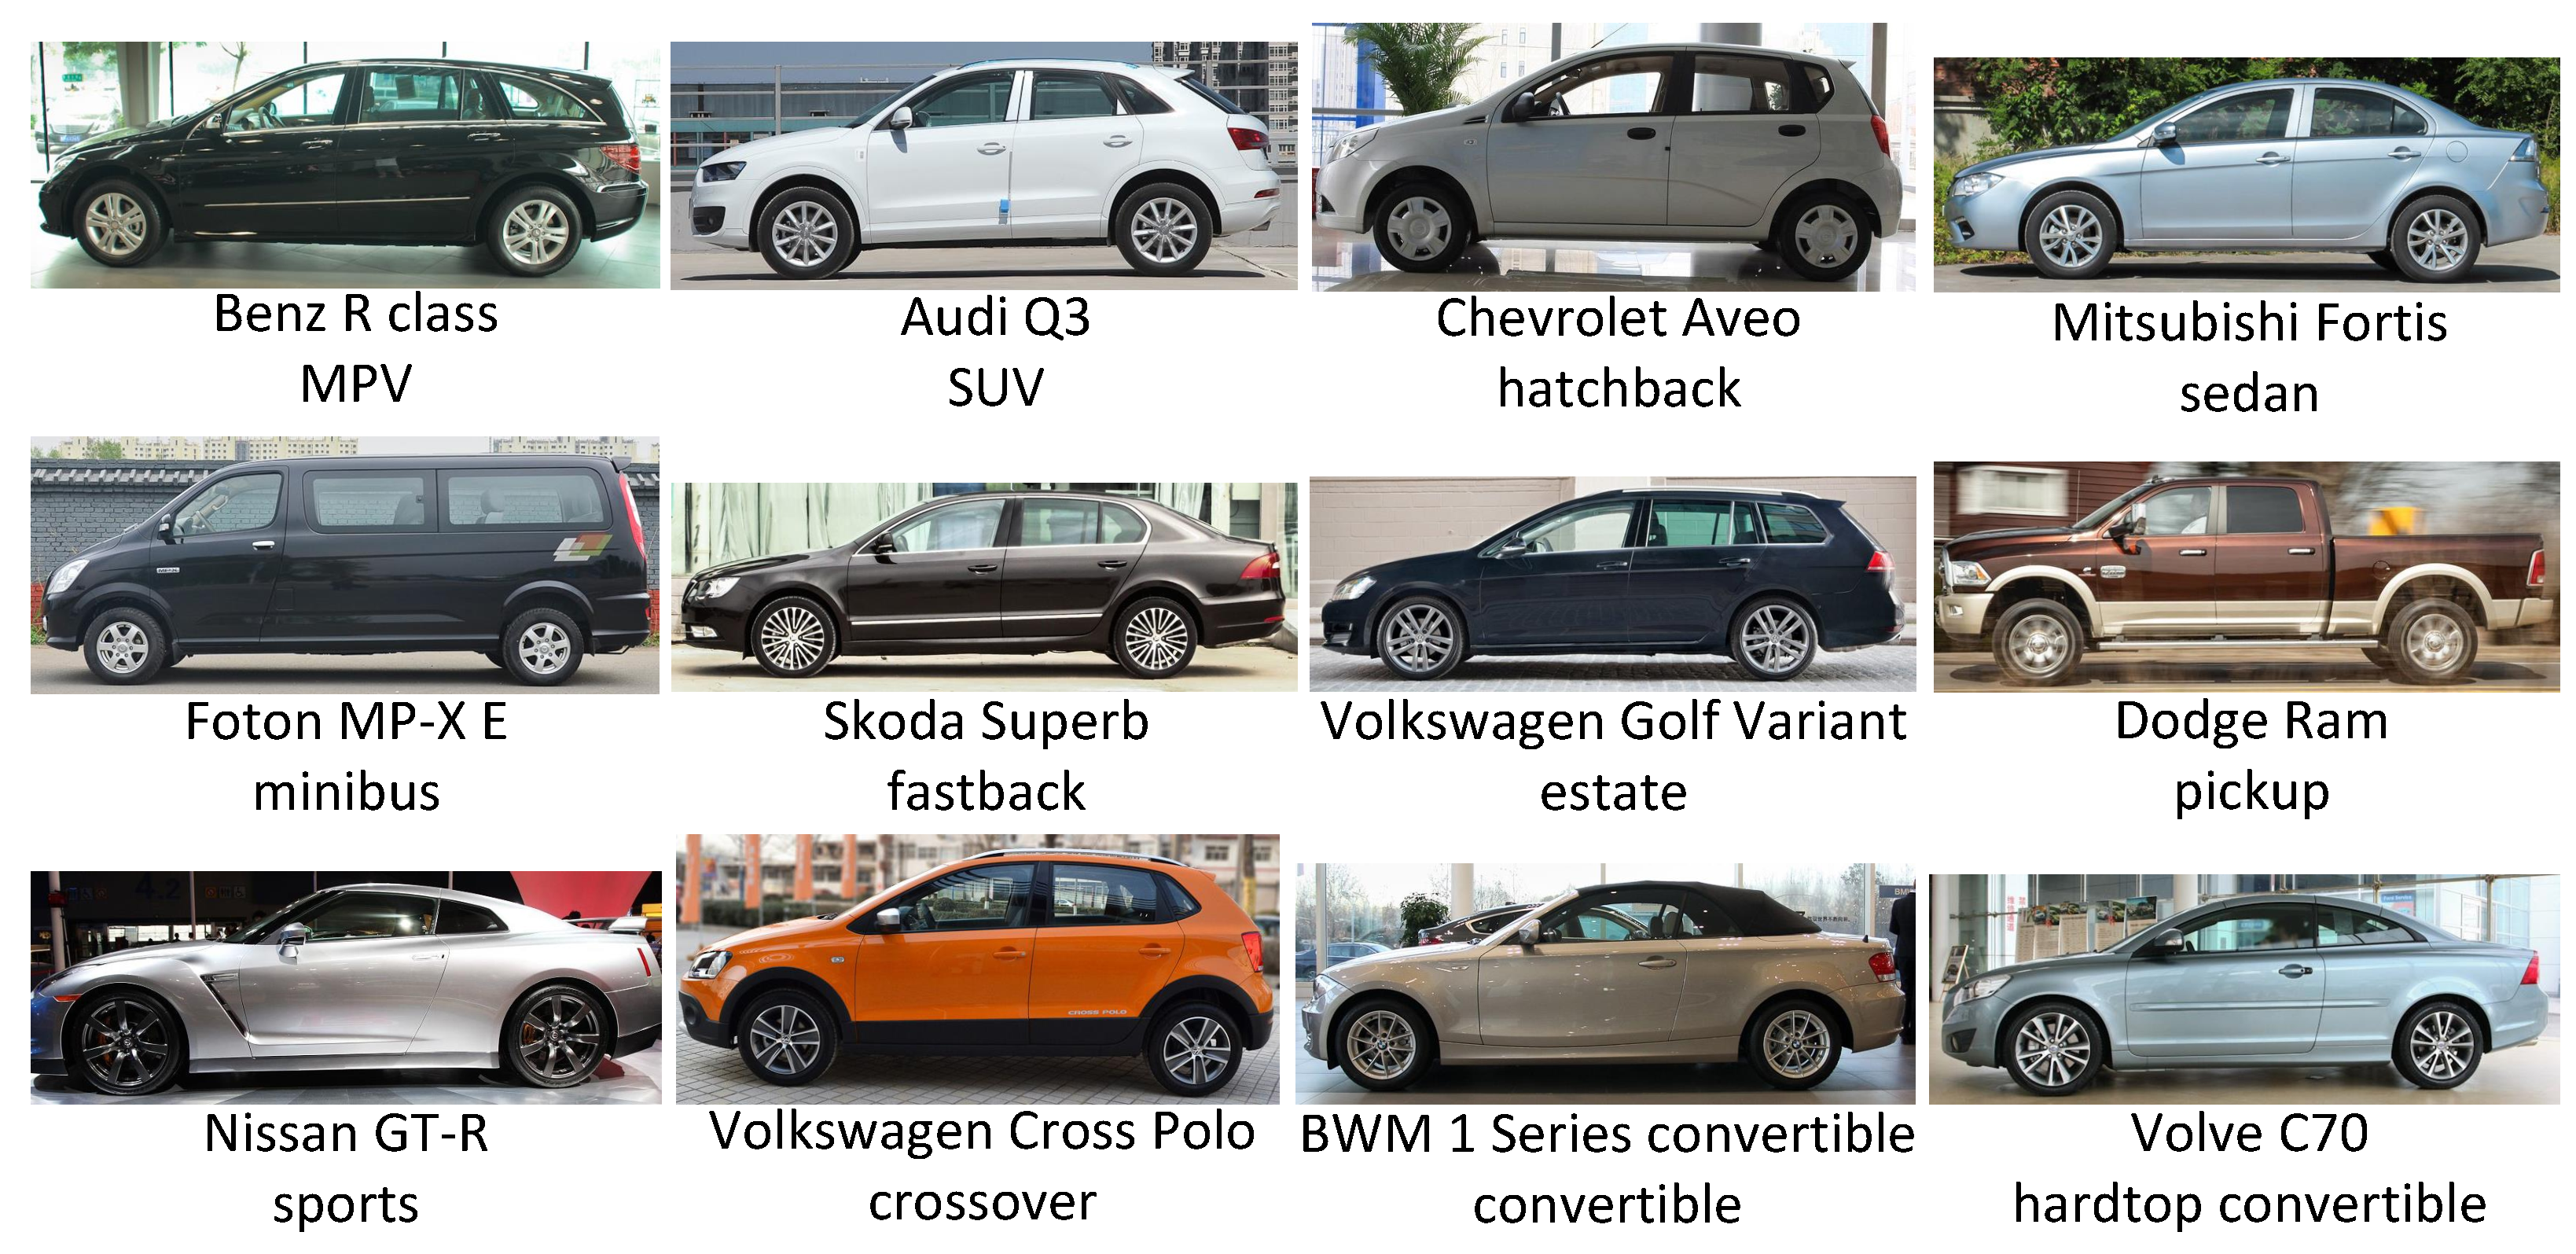
\includegraphics[width=1\linewidth]{type.pdf}
\caption{Each image displays a car from the 12 car types. The corresponding model names and car types are shown below the images.}
\label{fig:type}
\vspace{-4pt}
\end{figure}

\textbf{Car Attributes}
Each car model is labeled with five attributes, including maximum speed, displacement, number of doors, number of seats, and type of car. These attributes provide rich information while learning the relations or similarities between different car models.
%
For example, we define twelve types of cars, which are MPV, SUV, hatchback, sedan, minibus, fastback, estate, pickup, sports, crossover, convertible, and hardtop convertible, as shown in Fig.~\ref{fig:type}.
%
Furthermore, these attributes can be partitioned into two groups: explicit and implicit attributes. The former group contains door number, seat number, and car type, which are represented by discrete values, while the latter group contains maximum speed and displacement (volume of an engine's cylinders), represented by continuous values.
%
Humans can easily tell the numbers of doors and seats from a car's proper viewpoint, but hardly recognize its maximum speed and displacement.
%
We conduct interesting experiments to predict these attributes in Section~\ref{sec:attr}.


%Among the attributes, maximum speed and displacement are continuous values, while door number, seat number, and car type are discrete values. The rich attributes can provide essential information while learning the relationship or similarity between different car models.
%
%They can also be learned directly from the images.
%
%Humans can easily tell how many doors and seats one car has from a proper view of the car. But for maximum speed or displacement, non-expertise cannot give an accurate prediction with only an image displaying the car. So we also classifies the attributes into two groups: explicit and implicit. All three discrete attributes belong to the explicit attributes while both two continuous attributes belong to the implicit attributes.

\textbf{Viewpoints}
We also label five viewpoints for each car model, including front (F), rear (R), side (S), front-side (FS), and rear-side (RS). These viewpoints are labeled by several professional annotators. The quantity distribution of the labeled car images is shown in Table~\ref{tab:dist_view}.
%
Note that the numbers of viewpoint images are not balanced among different car models, because the images of some less popular car models are difficult to collect.

%%equalized from different models since the images of models are harder to collect and have smaller quantities. Extracting subsets could be a proper way to conduct the experiments which prefer more images for each model.

%Each model has car images annotated in 5 viewpoints: front (F), rear (R), side (S), front-side (FS), and rear-side (RS).
%
%The first three viewpoints, front, rear, and side has relatively narrow viewpoint ranges. For example, if the viewpoint of a car is deviated from right front by more than $10^\circ$, it is labeled as front-side.
%
%The viewpoints of the car images are labeled by several workers and double-checked by the authors. The quantity distribution of the labeled car images is shown in Table~\ref{tab:dist_view}. Every car image is labeled with viewpoint except for 60 images that have irregular viewpoints (e.g. a top view).

%Notice that the image numbers are not equalized from different models since the images of unpopular models are harder to collect and have smaller quantities. Extracting subsets could be a proper way to conduct the experiments which prefer more images for each model.

\begin{table}
\small
\centering
\caption{Quantity distribution of the labeled car images in different viewpoints.}
\begin{tabular}{*{3}{|c}|}
\hline
Viewpoint & No. in total  & No. per model \\
\hline
F & 18431 & 10.9\\
\hline
R & 13513 & 8.0\\
\hline
S & 23551 & 14.0\\
\hline
FS & 49301 & 29.2\\
\hline
RS & 31150 & 18.5\\
\hline
\end{tabular}
\label{tab:dist_view}
\vspace{-3pt}
\end{table}

\begin{table}
\small
\centering
\caption{Quantity distribution of the labeled car part images.}
\begin{tabular}{*{3}{|c}|}
\hline
Part & No. in total  & No. per model \\
\hline
headlight & 3705 &	2.2  \\
 \hline
 taillight & 3563 & 2.1 \\
 \hline
 fog light & 3177 &	1.9  \\
 \hline
 air intake & 3407 & 2.0	 \\
 \hline
 console & 3350 &	2.0  \\
 \hline
 steering wheel & 3503 & 2.1 \\
 \hline
 dashboard & 3478 &	2.1  \\
 \hline
 gear lever & 3435 & 2.0 \\
\hline

\end{tabular}
\label{tab:dist_part}
\vspace{-3pt}
\end{table}

\textbf{Car Parts}
We collect images capturing the eight car parts for each car model, including four exterior parts (\ie headlight, taillight, fog light, and air intake) and four interior parts (\ie console, steering wheel, dashboard, and gear lever). These images are roughly aligned for the convenience of further analysis.
%
A summary and some examples are given in Table~\ref{tab:dist_part} and Fig.~\ref{fig:part} respectively.

%Each model has images of 4 exterior car parts () and 4 interior car parts (console, steering wheel, dashboard, and gear lever).
%
%The car parts are selected by their quantity and discriminative ability for car models. The car part images are weakly aligned for the convenience of further analysis. The quantity distribution of the car part images is shown in Table~\ref{tab:dist_part}. The sample images are shown in Fig.~\ref{fig:interest} and Fig.~\ref{fig:part}.
%height, width, length, maximum speed, displacement, door number, seat number, car type
%continuous attributes, discrete attributes
%attributes can provide side information when one tries to learn the relationship or similarity between different models.
%It can also be learned with the training data. We conduct an interesting experiment of predict the attributes on novel car models in Section~\ref{}.


\section{Applications}\label{sec:exp}

In this section, we study three applications using \datasetName{}, including fine-grained car classification, attribute prediction, and car verification.
%
We select $78,126$ images from the \datasetName{} dataset and divide them into three subsets without overlaps. The first subset (Part-I) contains $431$ car models with a total of $30,955$ images capturing the entire car and $20,349$ images capturing car parts. The second subset (Part-II) consists $111$ models with $4,454$ images in total. The last subset (Part-III) contains $1,145$ car models with $22,236$ images.
%
Fine-grained car classification is conducted using images in the first subset. For attribute prediction, the models are trained on the first subset but tested on the second one. The last subset is utilized for car verification.

%. The first experiment is the fine-grained classification of car models with car images or car part images. The second experiment is attribute prediction from novel car models. The last experiment is car model verification.
%
%\textcolor{red}{We use a subset of 78,669 images from the dataset and divide the data into three parts}: Part-I is 431 models for fine-grained classification, Part-II is 111 models for the training of car model verification, and Part-III is the other 1,145 models for the testing of car model verification.
%
%Since image numbers for different models are not balanced in our dataset, the division is conducted under the guideline that Part-I has more images for each model, which is proper to verify the effectiveness of the fine-grained classification model. The image numbers of cars for the three parts are 31,322, 4,493, and 22,373, respectively. An extra number of 20,481 car part images are used for Part-I. The attribute prediction models are trained on Part-I and tested on Part-II.

%In this section, we show three applications on \datasetName{}. The first experiment is the fine-grained classification of car models with car images or car part images. The second experiment is attribute prediction from novel car models. The last experiment is car model verification. \textcolor{red}{We use a subset of 78,669 images from the dataset and divide the data into three parts}: Part-I is 431 models for fine-grained classification, Part-II is 111 models for the training of car model verification, and Part-III is the other 1,145 models for the testing of car model verification. Since image numbers for different models are not balanced in our dataset, the division is conducted under the guideline that Part-I has more images for each model, which is proper to verify the effectiveness of the fine-grained classification model. The image numbers of cars for the three parts are 31,322, 4,493, and 22,373, respectively. An extra number of 20,481 car part images are used for Part-I. The attribute prediction models are trained on Part-I and tested on Part-II.

\begin{figure}[t]\centering
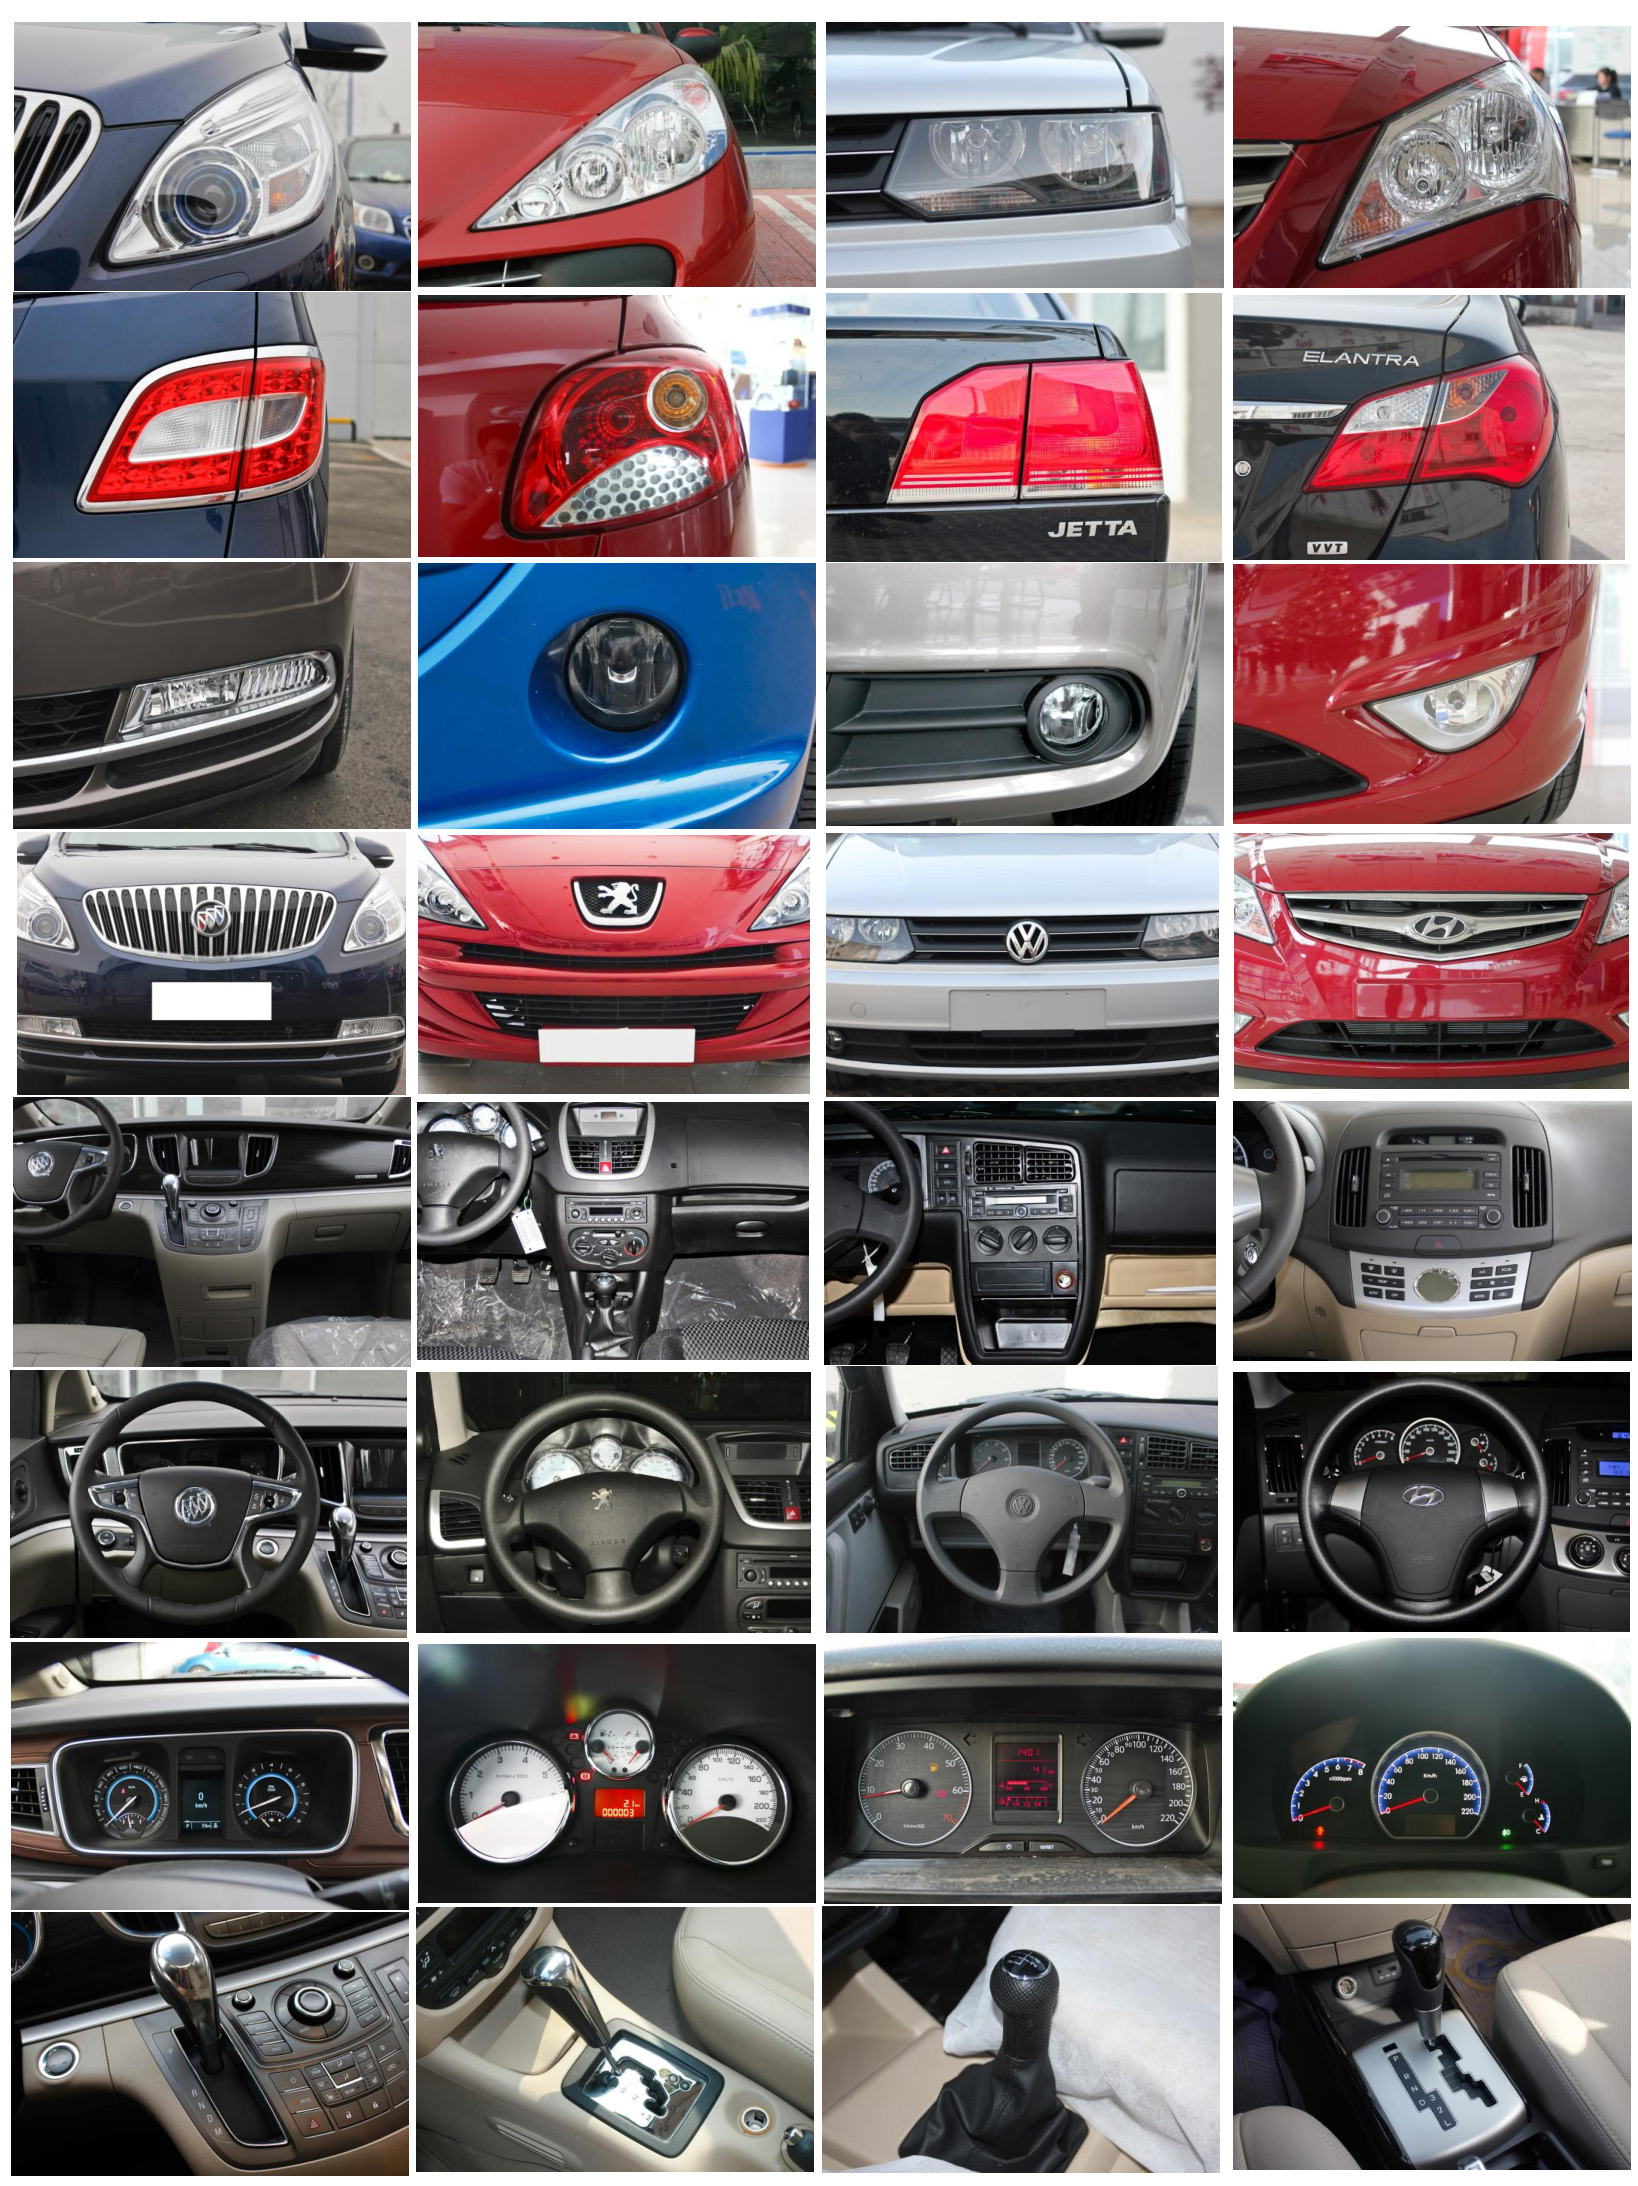
\includegraphics[width=0.9\linewidth]{part.pdf}
\caption{Each column displays 8 car parts from a car model. The corresponding car models are Buick GL8, Peugeot 207 hatchback, Volkswagen Jetta, and Hyundai Elantra from left to right, respectively.}
\label{fig:part}
\vspace{-3pt}
\end{figure}

We investigate the above potential applications using Convolutional Neural Network (CNN), which achieves great empirical successes in many computer vision problems, such as object classification~\cite{Krizhevsky12}, detection~\cite{rcnn14}, face alignment~\cite{ZhangECCV2014}, and face verification~\cite{Sun14,ZhuNIPS2014}.
%
Specifically, we employ the Overfeat~\cite{Sermanet13} model, which is pretrained on ImageNet classification task~\cite{Deng09}, and fine-tuned with the car images for car classification and attribute prediction. For car model verification, the fine-tuned model is employed as a feature extractor.

%The convolutional neural network has gained a wide variety of successes in object classification~\cite{Krizhevsky12},~\cite{He14spp},~\cite{Deng14} object detection~\cite{rcnn14}~\cite{Ouyang13}~\cite{Yang14}, face verification~\cite{Sun14}~\cite{Taigman14}, depth map prediction~\cite{Eigen14}, and so on.

%CNN models pretrained on ImageNet classification task~\cite{Deng09} are adopted to leverage the rich knowledge of ImageNet for lots of nature image based applications~\cite{Donahue13}~\cite{rcnn14}~\cite{Eigen14}. We fine-tune Overfeat~\cite{Sermanet13}, a CNN model which is pretrained on ImageNet, for each task in the fine-grained classification and the attribute prediction sections. For car model verification, the fine-tuned classification model is acted as a feature extractor. All images are resized to 256$\times$256 pixels to fit the input of the Overfeat model.


\subsection{Fine-Grained Classification}

We classify the car images into $431$ car models. For each car model, the car images produced in different years are considered as a single category. One may treat them as different categories, leading to a more challenging problem because their differences are relatively small.
%
%Our target in this section is fine-grained classification of 431 car models with the images in \datasetName{}. We do not consider the year level difference for car models as Krause et al.~\cite{Krause13} here since year level difference is relatively subtle in comparison with the model level difference.
Our experiments have two settings, comprising fine-grained classification with the entire car images and the car parts. For both settings, we divide the data into half for training and another half for testing.
Car model labels are regarded as training target and logistic loss is used to fine-tune the Overfeat model.
%All experiments in this section divide the train and test datasets in a 50\%/50\% fashion.


\subsubsection{The Entire Car Images}\label{sec:cls}

We compare the recognition performances of the CNN models, which are fine-tuned with car images in specific viewpoints and all the viewpoints respectively, denoted as ``front (F)'', ``rear (R)'', ``side (S)'', ``front-side (FS)'', ``rear-side (RS)'', and ``All-View''.
%
The performances of these six models are summarized in Table~\ref{tab:cls_car}, where ``FS'' and ``RS'' achieve better performances than the performances of the other viewpoint models.
%
Surprisingly, the ``All-View'' model yields the best performance, although it did not leverage the information of viewpoints. This result reveals that the CNN model is capable of learning discriminative representation across different views.
%
To verify this observation, we visualize the car images that trigger high responses with respect to each neuron in the last fully-connected layer. As shown in Fig.~\ref{fig:response}, these neurons capture car images of specific car models across different viewpoints.

%targets at a more complex problem. \textcolor{red}{The All-View achieves the best performance because it is capable of learning shared representation across different views. From our observation, some neurons in the last fully connected layer of the CNN model actually give high responses to certain car models under different views. Fig.~\ref{fig:response} shows images having highest responses from two sample neurons, which belong to a same model, respectively.}
%
%The appearances in different viewpoints also carry different information of the car model. In this section, we conduct fine-grained classification experiments for the five labeled viewpoints: front (F), rear (R), side (S), front-side (FS), and rear-side (RS). We also train a model with all the car images without viewpoint annotations, which is denoted as \emph{All-View} for short.
%
%The performance of the six models is shown in Table~\ref{tab:cls_car}. For the models targeted at different viewpoints, the models for the viewpoints FS and RS gain better performance than the other models, partially because there are more images under these two viewpoints.
%
%To our surprise, the All-View model yields the best performance, although it targets at a more complex problem. \textcolor{red}{The All-View achieves the best performance because it is capable of learning shared representation across different views. From our observation, some neurons in the last fully connected layer of the CNN model actually give high responses to certain car models under different views. Fig.~\ref{fig:response} shows images having highest responses from two sample neurons, which belong to a same model, respectively.}

\begin{figure}[t]\centering
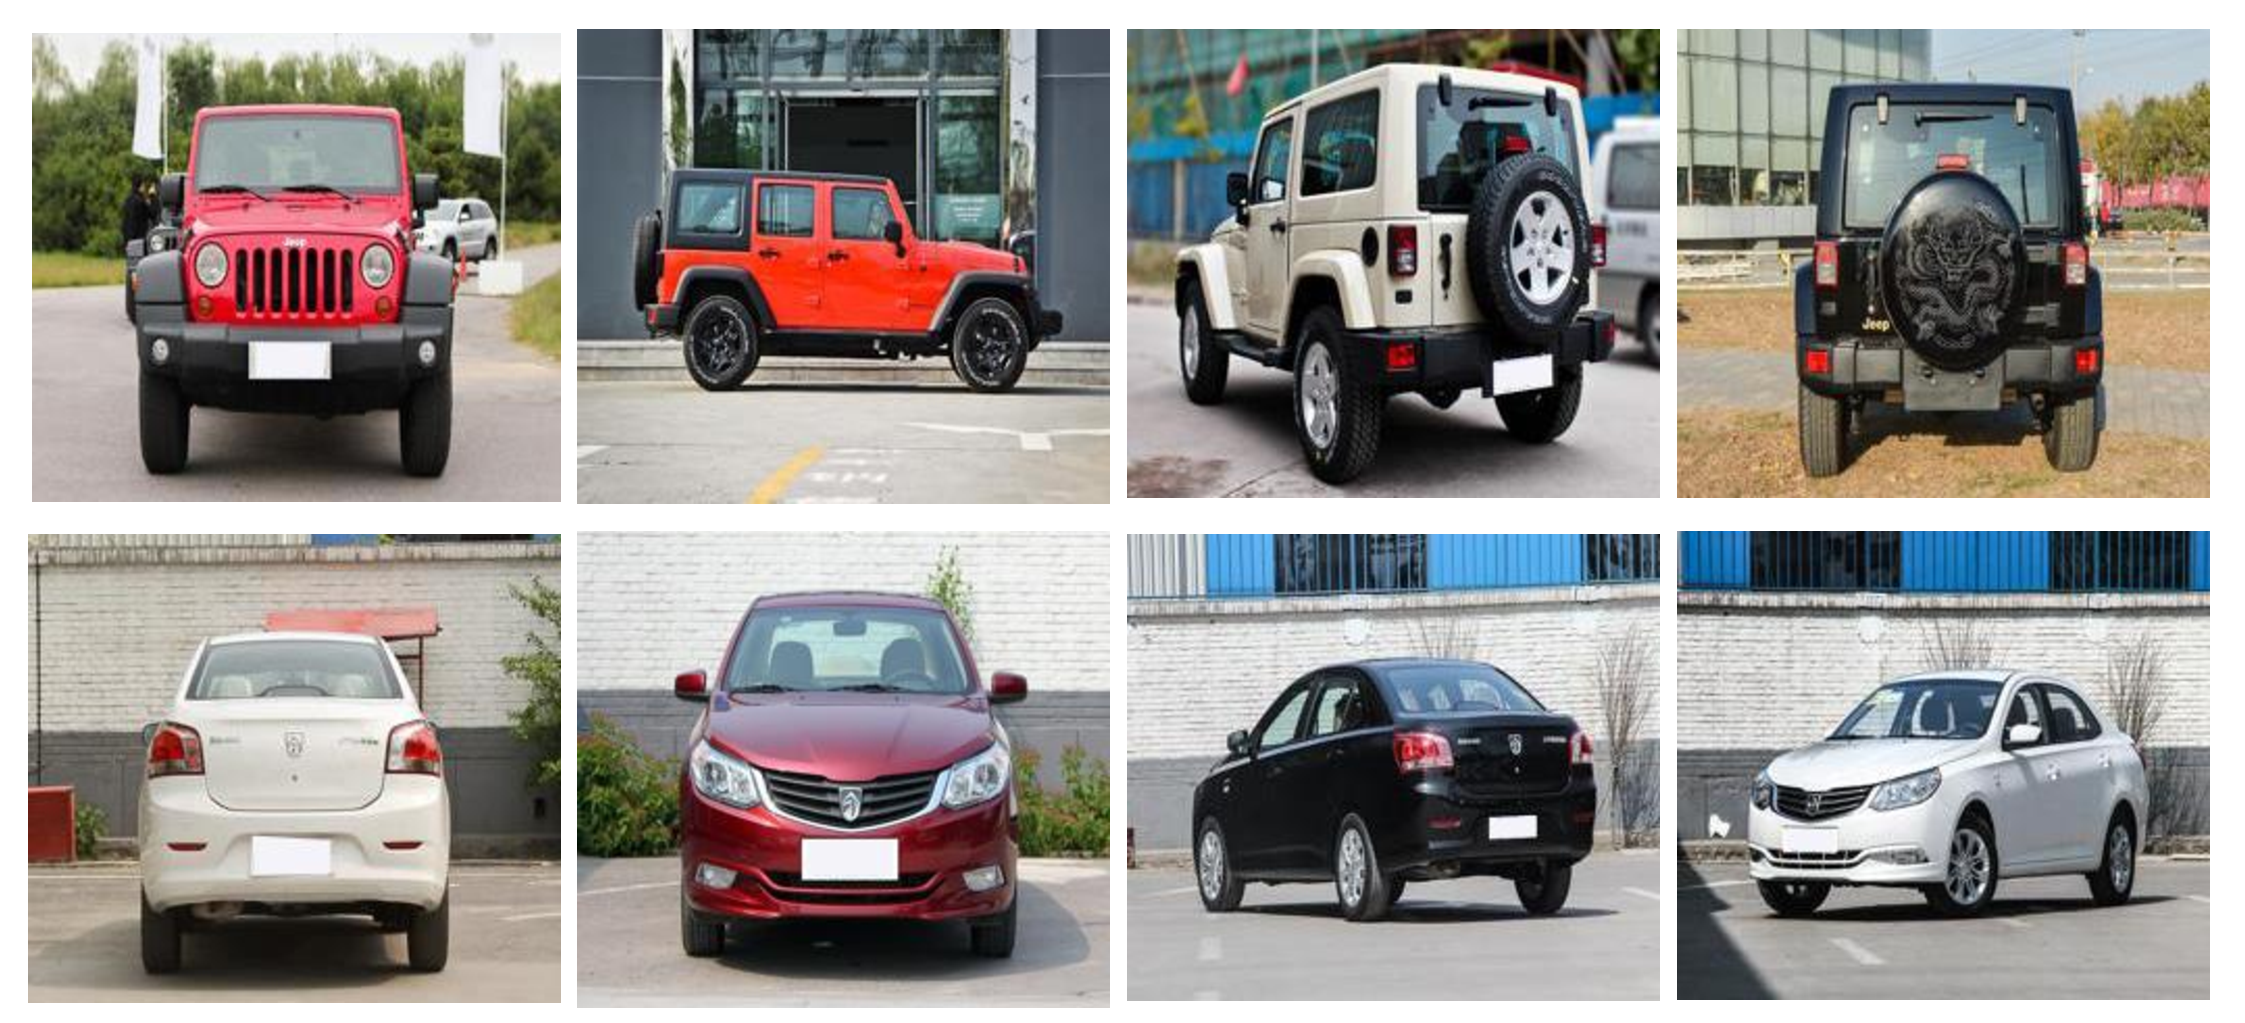
\includegraphics[width=1\linewidth]{response.pdf}
\caption{Images with the highest responses from two sample neurons. Each row corresponds to a neuron.}
\label{fig:response}
\vskip -0.35cm
\end{figure}

\begin{figure}[t]\centering
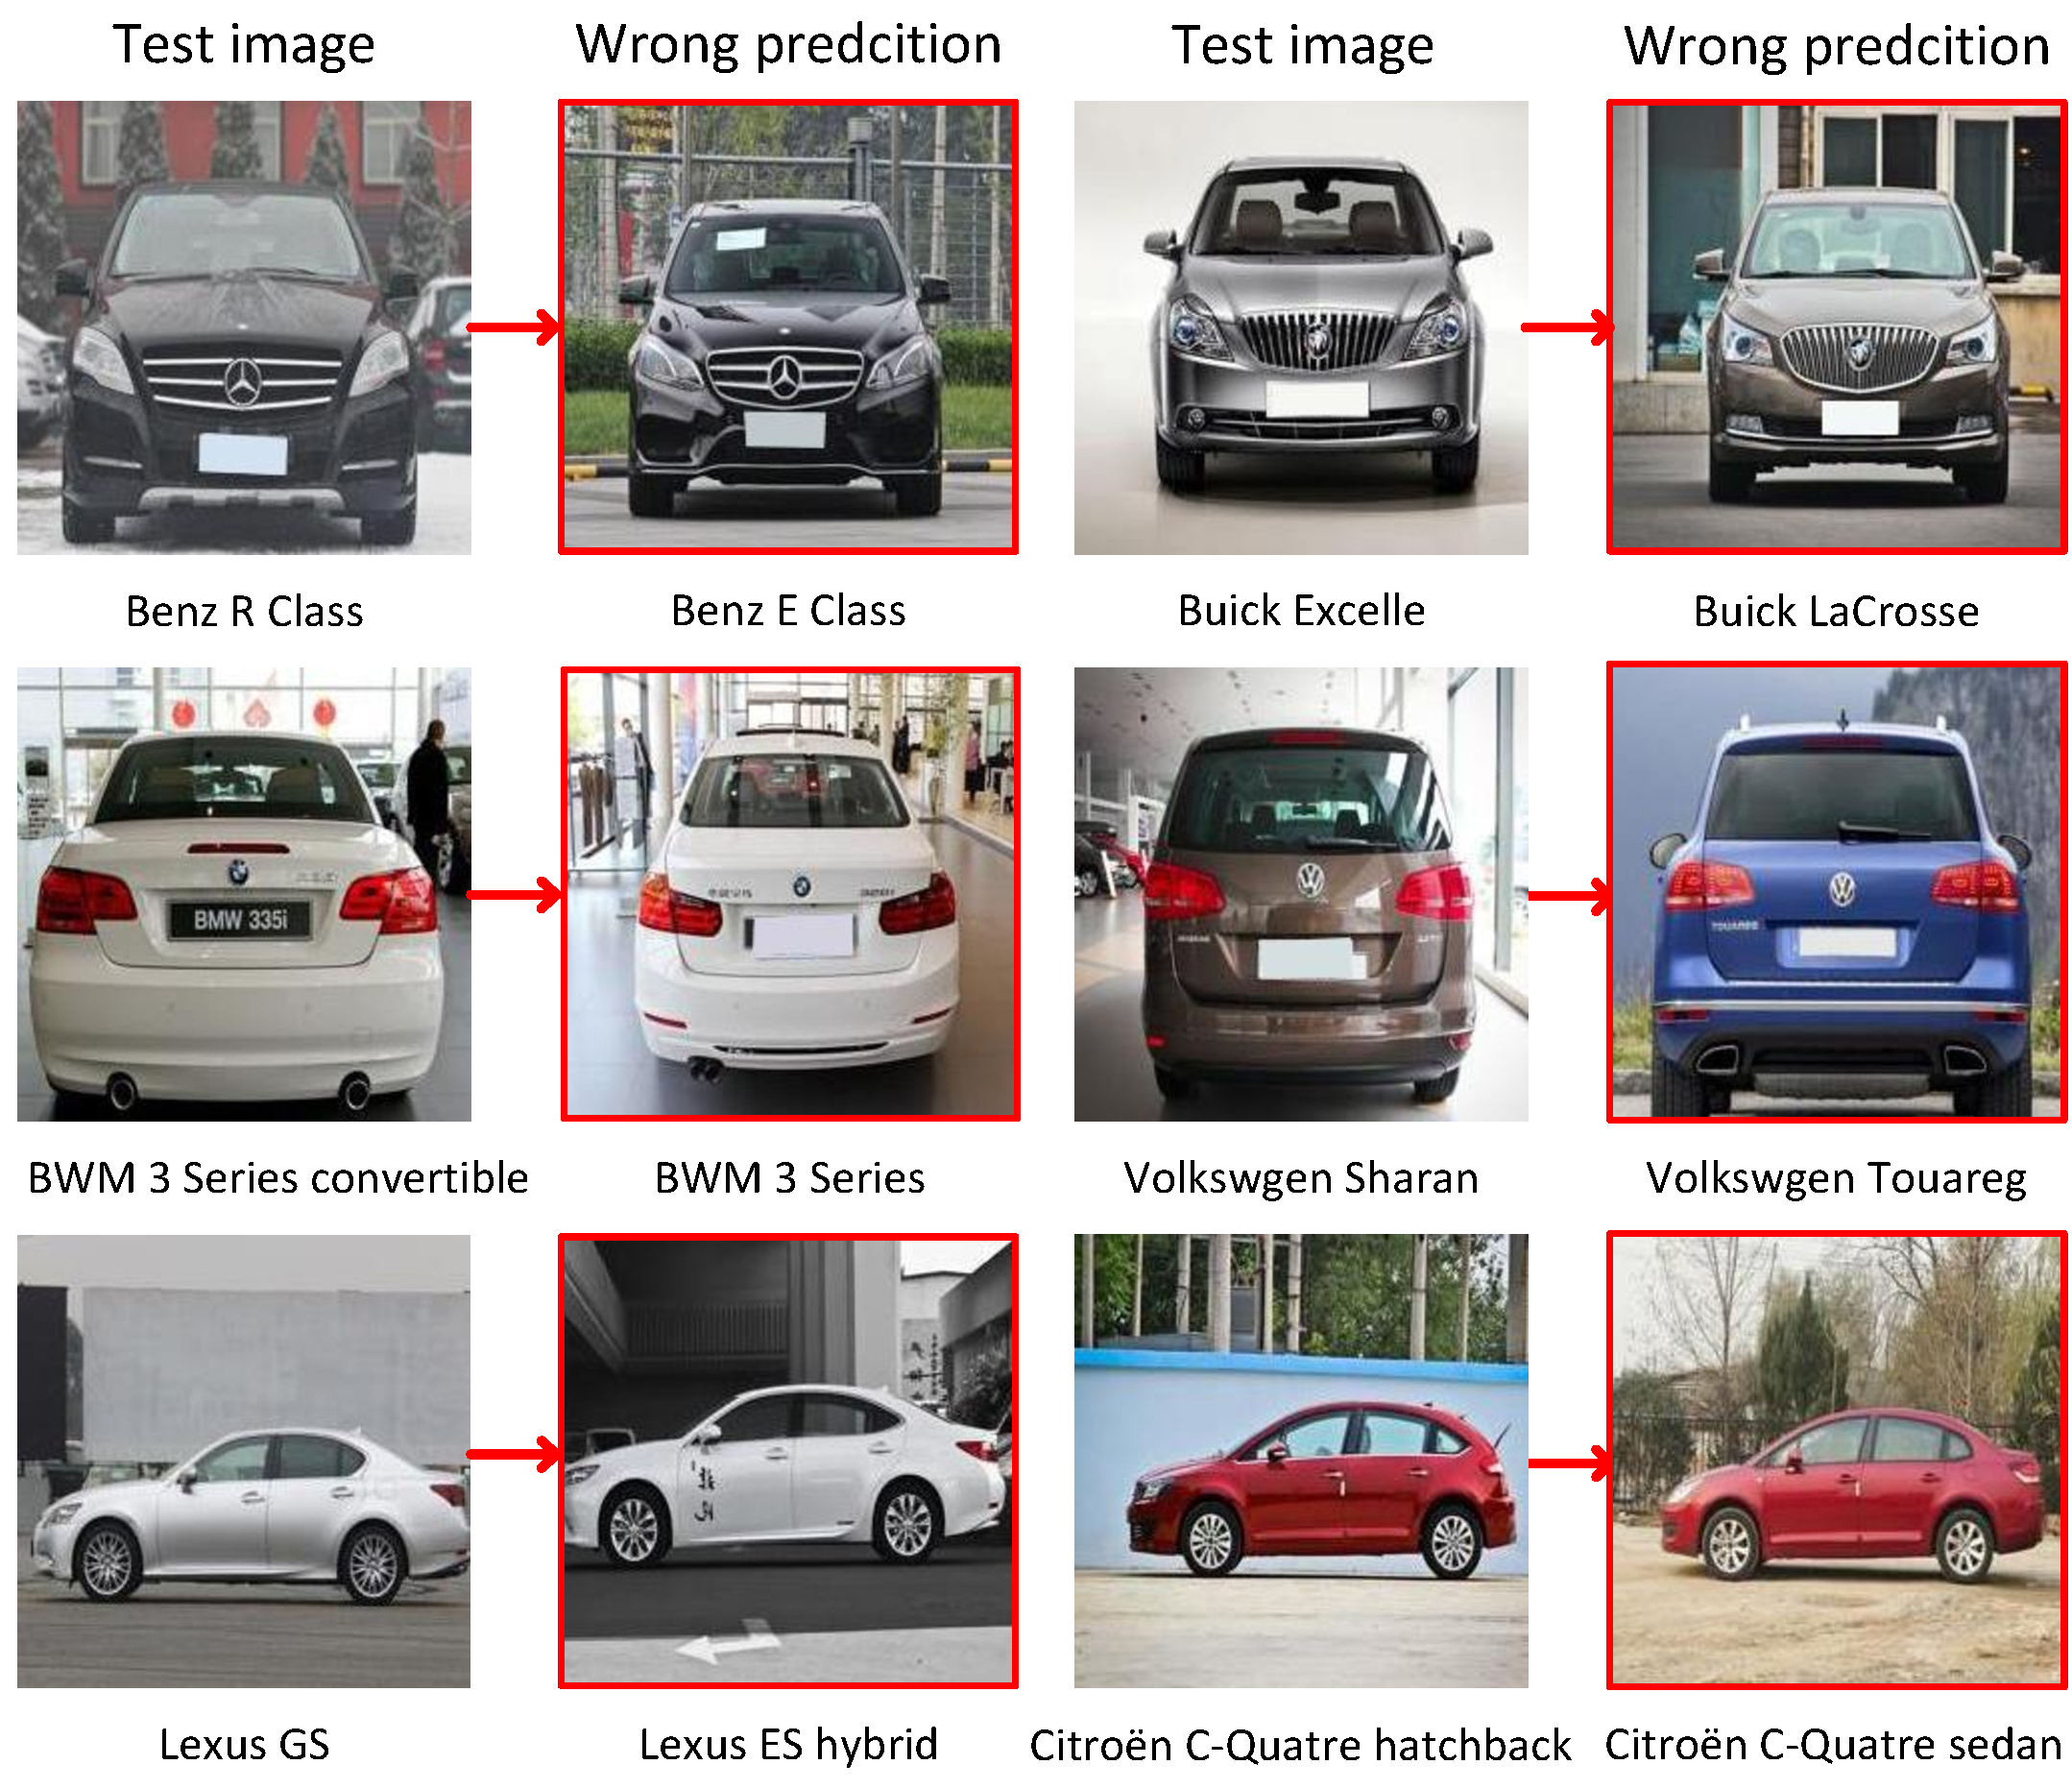
\includegraphics[width=1\linewidth]{cls_err.pdf}
\caption{Sample test images that are mistakenly predicted as another model in their makes. Each row displays two samples and each sample is a test image followed by another image showing its mistakenly predicted model. The corresponding model name is shown under each image.}
\label{fig:cls_err}
\vspace{-3pt}
\end{figure}

\begin{figure}[t]\centering
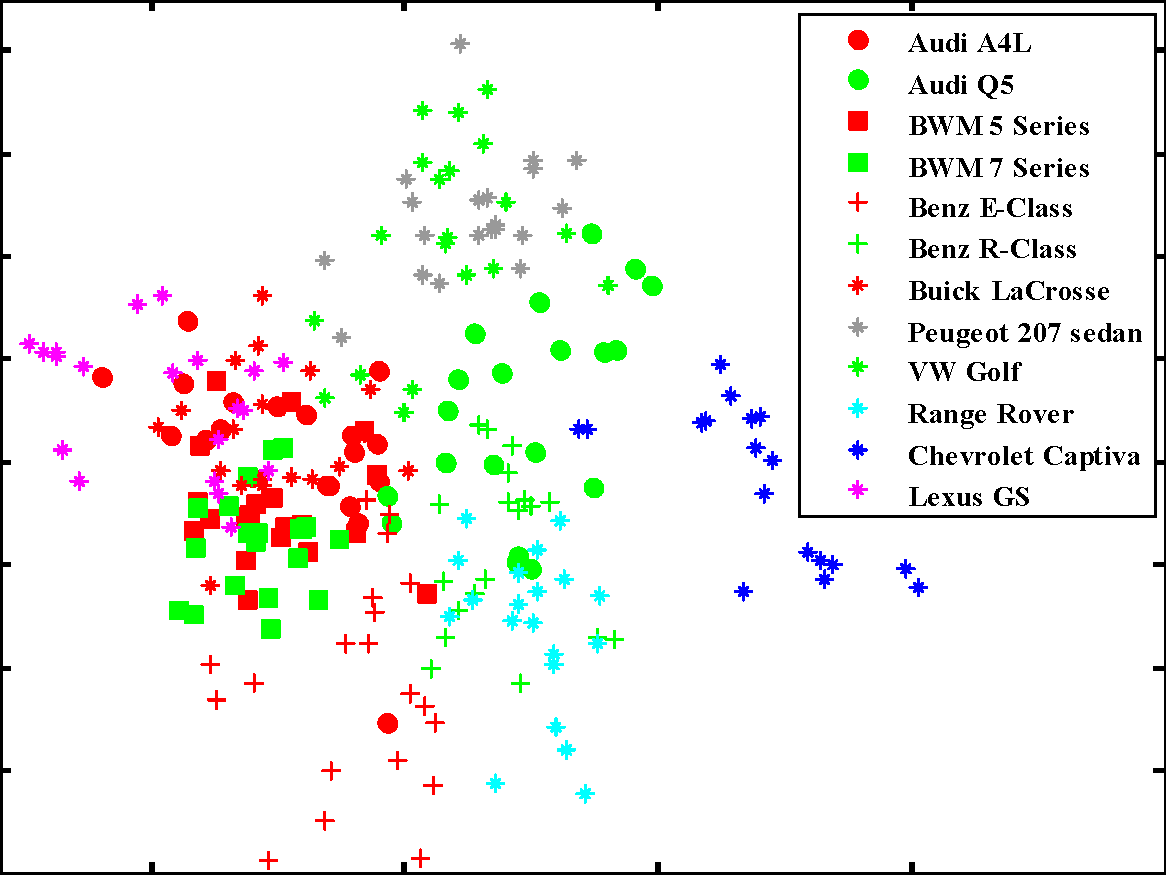
\includegraphics[width=1.0\linewidth]{sample_dist.pdf}
\caption{The features of 12 car models that are projected to a two-dimensional embedding using multi-dimensional scaling. Most features are separated in the 2D plane with regard to different models. Features extracted from similar models such as BWM 5 Series and BWM 7 Series are close to each other. Best viewed in color.}
\label{fig:dist}
\vskip -0.35cm
\end{figure}

Several challenging cases are given in Fig.~\ref{fig:cls_err}, where the images on the left hand side are the testing images and the images on the right hand side are the examples of the wrong predictions (of the ``All-View'' model). We found that most of the wrong predictions belong to the same car makes as the test images.
%
%Fig.~\ref{fig:cls_err} shows several challenging test images, which are mistakenly predicted as another model in their makes with the All-View model.\
%
We report the ``top-1'' accuracies of car make classification in the last row of Table~\ref{tab:cls_car}, where the ``All-View'' model obtain reasonable good result, indicating that a coarse-to-fine (\ie from car make to model) classification is possible for fine-grained car recognition.

%Browsing the incorrect test samples, we find that a large portion of errors are due to inter-make confusions. Fig.~\ref{fig:cls_err} shows several challenging test images, which are mistakenly predicted as another model in their makes with the All-View model. We also display the make level accuracy in Table~\ref{tab:cls_car}. The inter-make similarities revealed by this experiment indicate that a hierarchical model may be preferred for car model classification.

To observe the learned feature space of the ``All-View'' model, we project the features extracted from the last fully-connected layer to a two-dimensional embedding space using multi-dimensional scaling. Fig.~\ref{fig:dist} visualizes the projected features of twelve car models, where the images are chosen from different viewpoints.
%
%Notice that the corresponding car images of the features are from different viewpoints.
We observe that features from different models are separable in the 2D space and features of similar models are closer than those of dissimilar models. For instance, the distances between ``BWM 5 Series'' and ``BWM 7 Series'' are smaller than those between ``BWM 5 Series'' and ``Chevrolet Captiva''. %The observations indicate the capability of the features for the verification task.
%% data equalization
\begin{table}
\small
\centering
\caption{Fine-grained classification results for the models trained on car images. Top-1 and Top-5 denote the top-1 and top-5 accuracy for car model classification, respectively. Make denotes the make level classification accuracy.}
\begin{tabular}{*{7}{|c}|}
\hline
 Viewpoint & F & R & S & FS & RS & All-View\\
\hline
Top-1 & 0.524 &	0.431 &	0.428 & 0.563 & 0.598 &	 0.767\\
Top-5 & 0.748 & 0.647 & 0.602 & 0.769 & 0.777 &  0.917\\
\hline
Make & 0.710 & 0.521 & 0.507 & 0.680 & 0.656 &  0.829\\
\hline
\end{tabular}
\label{tab:cls_car}
\vspace{-3pt}
\end{table}

%%cross modality experiment
We also conduct a cross-modality experiment, where the CNN model fine-tuned by the web-nature data is evaluated on the surveillance-nature data. Fig.~\ref{fig:cross_t5} illustrates some predictions, suggesting that the model may account for data variations in a different modality to a certain extent.
%
This experiment indicates that the features obtained from the web-nature data have potential to be transferred to data in the other scenario.

%We also conduct a qualitative experiment for the classification model trained on the web-nature data to be tested on the surveillance-nature data. Fig.~\ref{fig:cross_t5} illustrates the prediction results of the classification model for eight cars in the surveillance cameras. For all these samples, which are from different car makes and car types, the classification model can obtain reasonable predictions. This experiment indicates that the classification model trained on the web-nature data has the potential to be applied to data in other scenarios, which can yield a large visual gap from the web-nature images.

\begin{figure}[t]\centering
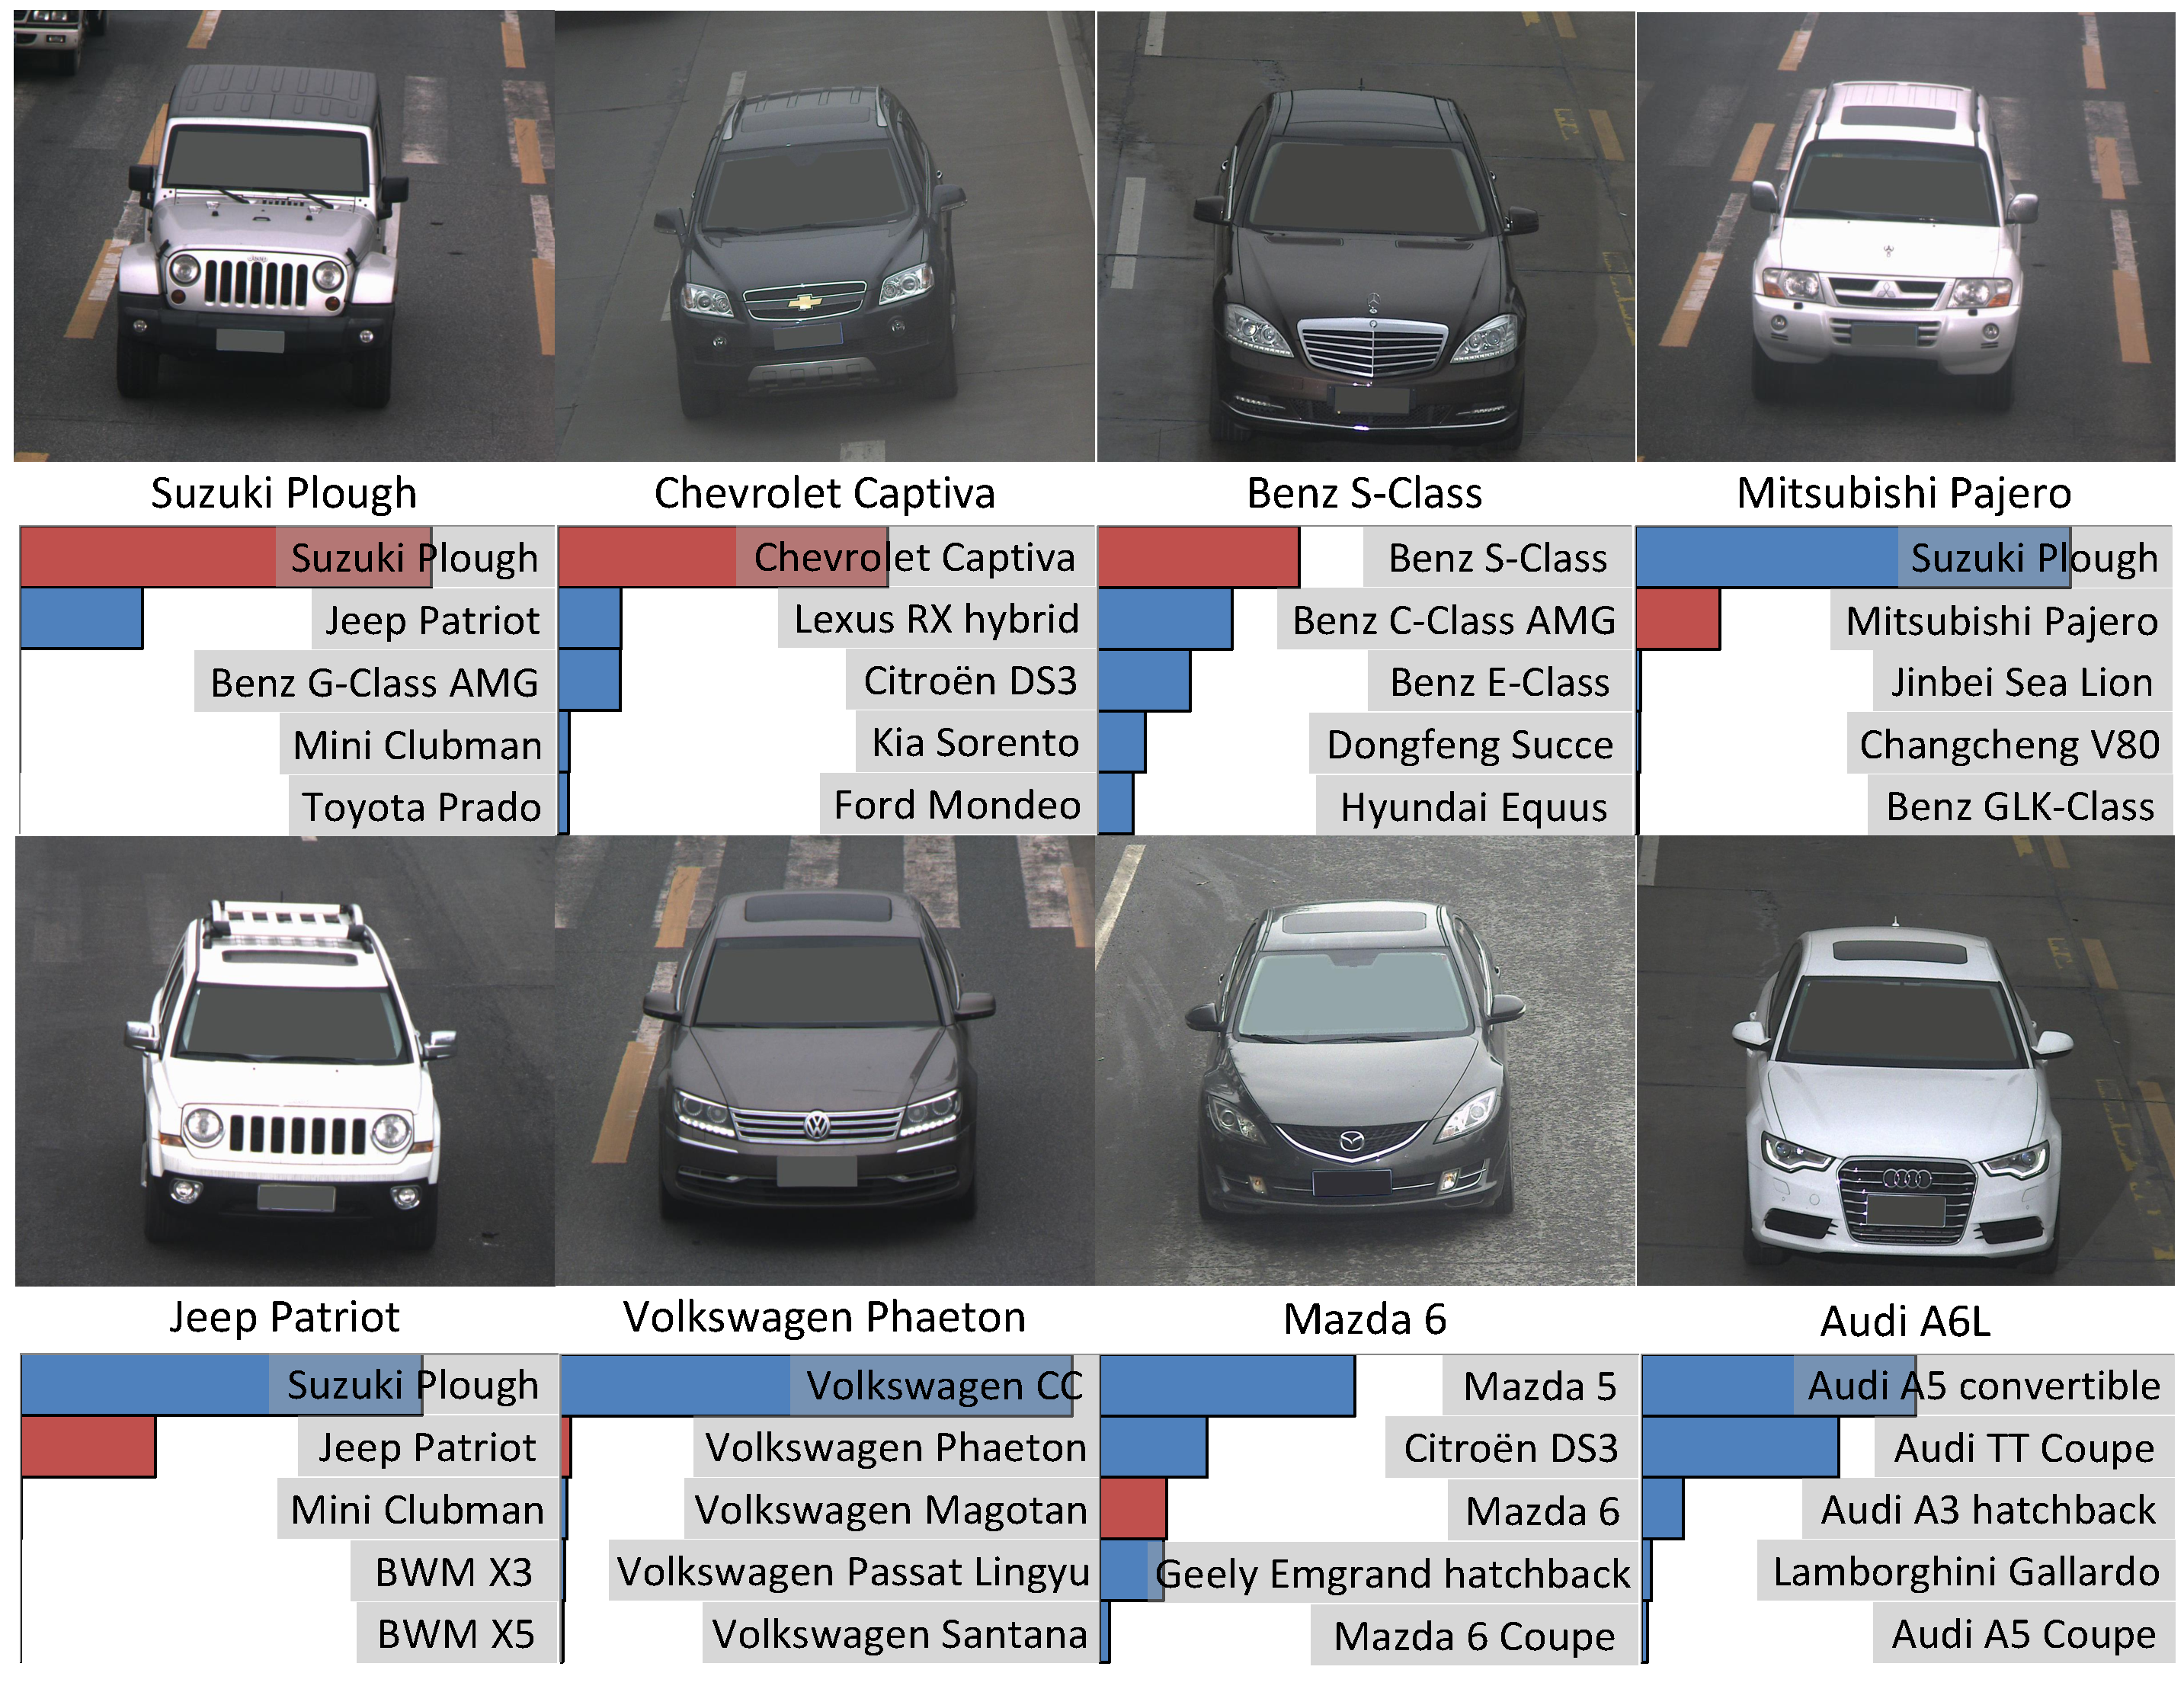
\includegraphics[width=1\linewidth]{cross_t5.pdf}
\caption{Top-5 predicted classes of the classification model for eight cars in the surveillance-nature data. Below each image is the ground truth class and the probabilities for the top-5 predictions with the correct class labeled in red. Best viewed in color.}
\label{fig:cross_t5}
\vspace{-3pt}
\end{figure}

\subsubsection{Car Parts}

Car enthusiasts are able to distinguish car models by examining the car parts. We investigate if the CNN model can mimic this strength.
%
We train a CNN model using images from each of the eight car parts. The results are reported in Table~\ref{tab:cls_part}, where ``taillight'' demonstrates the best accuracy.
%
We visualize taillight images that have high responses with respect to each neuron in the last fully-connected layer. Fig.~\ref{fig:part_response} displays such images with respect to two neurons. ``Taillight'' wins among the different car parts, mostly likely due to the relatively more distinctive designs, and the model name printed close to the taillight, which is a very informative feature for the CNN model.

%Car manufacturers usually print the model name close to the taillight, which is a very informative feature for the CNN model, and could be the key reason that ``taillight'' wins. To validate whether the model captures this information, we also visualize taillight images that have high responses with respect to each neuron in the last fully-connected layer. Fig.~\ref{fig:part_response} displays such images with respect to two neurons, indicating that the selected neurons have captured the information of the characters although they are not supervised to detect them.}

\begin{figure}[t]\centering
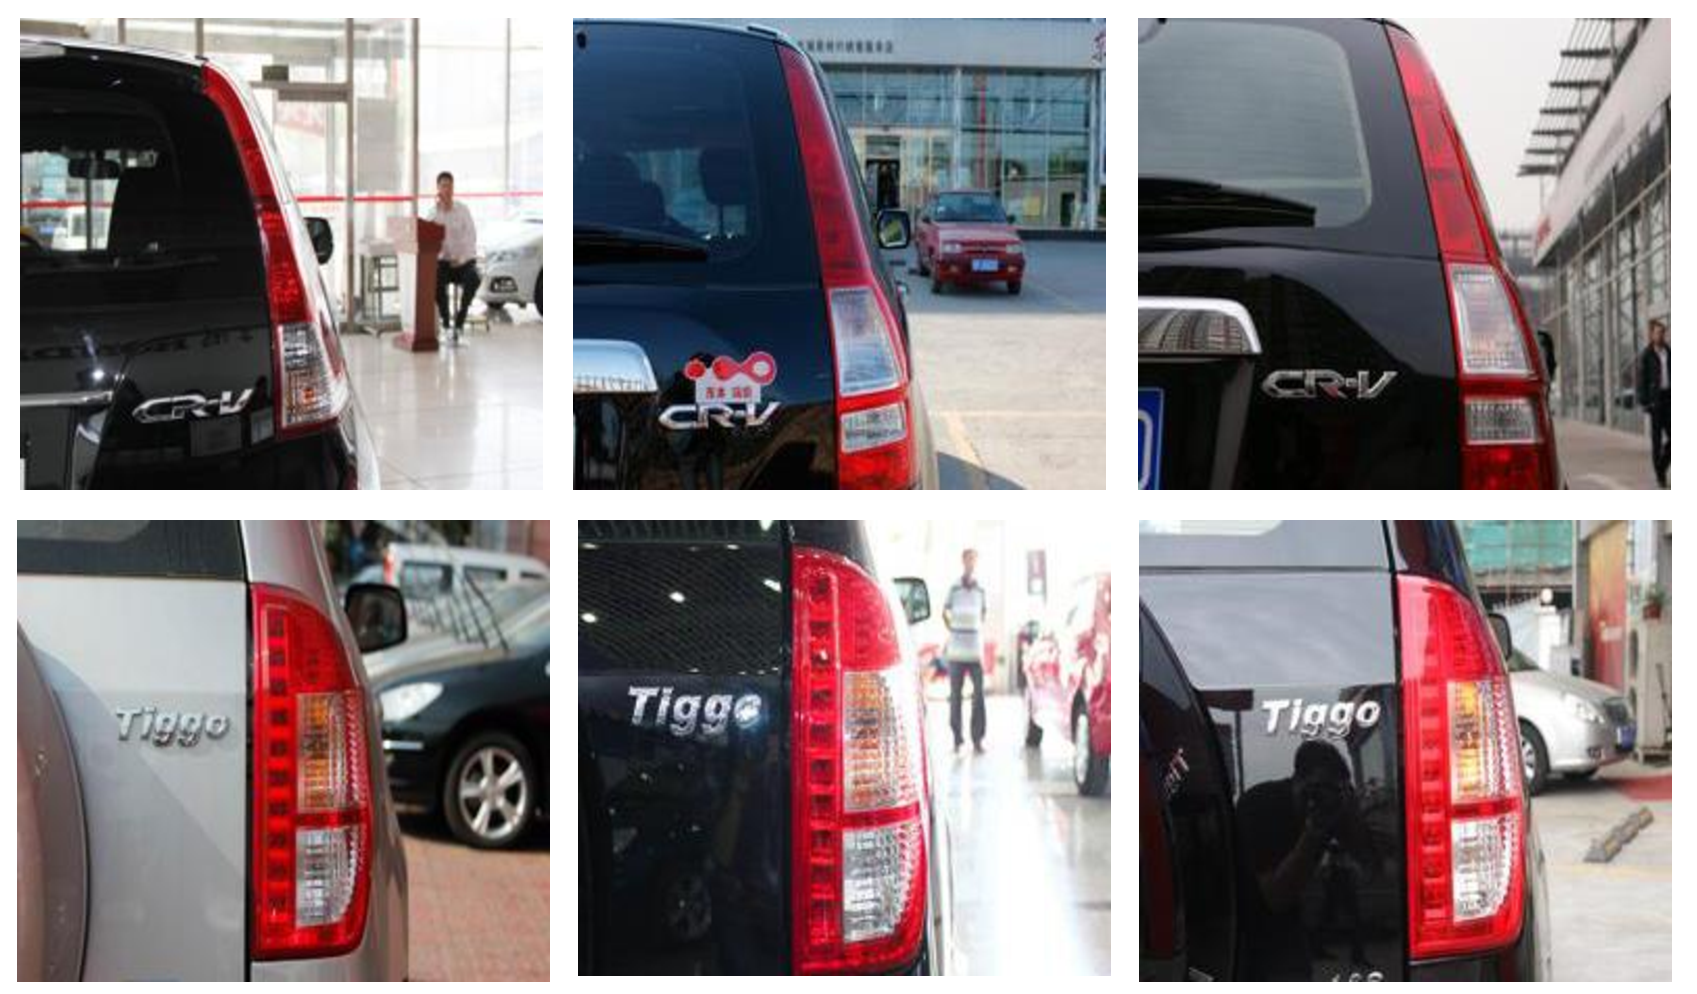
\includegraphics[width=0.7\linewidth]{part_response.pdf}
\caption{Taillight images with the highest responses from two sample neurons. Each row corresponds to a neuron.}
\label{fig:part_response}
\end{figure}
%
We also combine predictions using the eight car part models by voting strategy. This strategy significantly improves the performance due to the complementary nature of different car parts.


\begin{table*}
\small
\centering
\caption{Fine-grained classification results for the models trained on car parts. Top-1 and Top-5 denote the top-1 and top-5 accuracy for car model classification, respectively.}
\begin{tabular}{*{10}{|c}|}
\hline
& \multicolumn{4}{c|}{Exterior parts} & \multicolumn{4}{c|}{Interior parts} & \\
\cline{2-9}
  & Headlight & Taillight & Fog light & Air intake & Console & Steering wheel & Dashboard & Gear lever & Voting\\
\hline
Top-1 & 0.479 &0.684& 0.387& 0.484& 0.535& 0.540& 0.502& 0.355& 0.808 \\
\hline
Top-5 & 0.690 &0.859& 0.566 & 0.695& 0.745& 0.773& 0.736& 0.589& 0.927 \\
\hline
\end{tabular}
\label{tab:cls_part}
\vspace{-3pt}
\end{table*}

%%Observe the samples, get the response map and illustrate. Show classification samples, indicate that failed samples also obtain reasonable results.


\subsection{Attribute Prediction}\label{sec:attr}

\begin{figure}[t]\centering
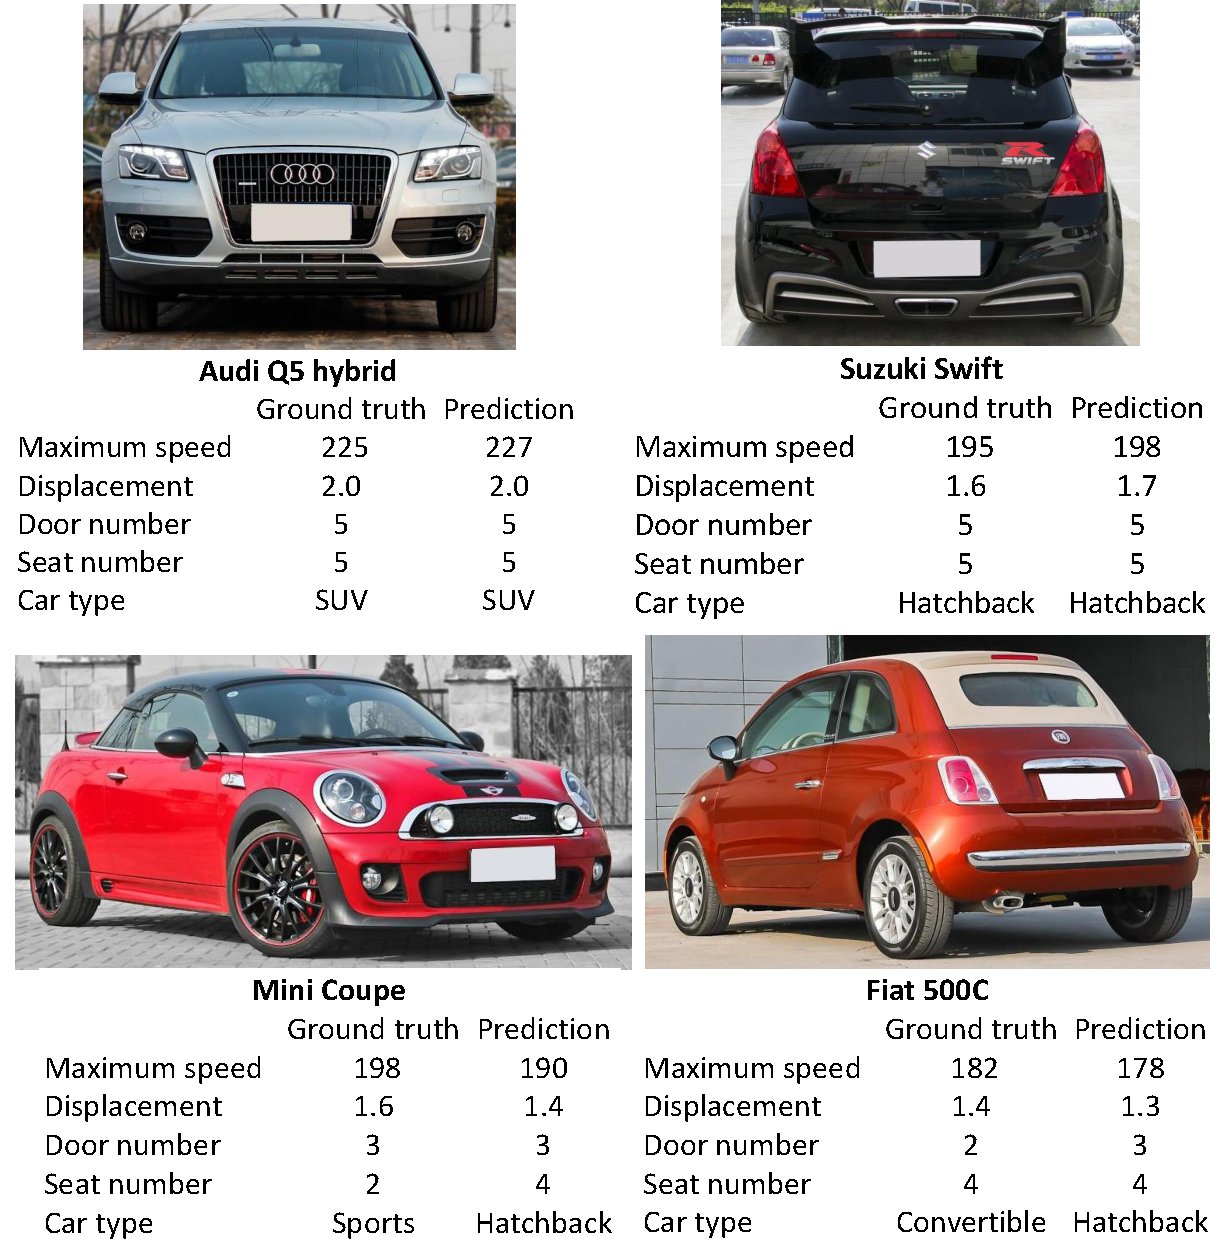
\includegraphics[width=0.9\linewidth]{attr.pdf}
\caption{Sample attribute predictions for four car images. The continuous predictions of maximum speed and displacement are rounded to nearest proper values.}
\label{fig:attr}
\vspace{-3pt}
\end{figure}

Human can easily identify the car attributes such as numbers of doors and seats from a proper viewpoint, without knowing the car model.
%
For example, a car image captured in the side view provides sufficient information of the door number and car type, but it is hard to infer these attributes from the frontal view.
%
The appearance of a car also provides hints on the implicit attributes, such as the maximum speed and the displacement. For instance, a car model is probably designed for high-speed driving, if it has a low under-pan and a streamline body.

In this section, we deliberately design a challenging experimental setting for attribute recognition, where the car models presented in the test images are exclusive from the training images.
%
We fine-tune the CNN with the sum-of-square loss to model the continuous attributes, such as ``maximum speed'' and ``displacement'', but a logistic loss to predict the discrete attributes such as ``door number'', ``seat number'', and ``car type''. For example, the ``door number'' has four states, \ie~$\left\{2, 3, 4, 5\right\}$ doors, while ``seat number'' also has four states, \ie~$\left\{2, 4, 5, >5\right\}$ seats. The attribute ``car type'' has twelve states as discussed in Sec.~\ref{sec:dataset}.

%classification model for the discrete attributes door number, seat number, and car type. The regression model utilizes sum-of-square loss whilst the classification one utilizes logistic loss. The door number attribute only has 4 unique values which represent 4 classes: 2, 3, 4, and 5. The seat number attribute is divided into 4 classes: 2, 4, 5, and more than 5. Car type is classified by its 12 classes.

%The task in this section is to train attribute prediction models and test them on novel car models.
%Without knowing the exact make and model, people can easily identify the explicit attributes of a car with a proper viewpoint. For example, a car in side view provides clear information of the door number and the car type of it. But it will be hard to infer these attributes with a front-view car.
%On the other hand, the appearance of a car also provides information on the implicit attributes: the maximum speed, the displacement, etc. With a low underpan and a streamline body, the car is probably designed for high speed driving.

%We train a regression model for the continuous attributes maximum speed and displacement, and a classification model for the discrete attributes door number, seat number, and car type. The regression model utilizes sum-of-square loss whilst the classification one utilizes logistic loss. The door number attribute only has 4 unique values which represent 4 classes: 2, 3, 4, and 5. The seat number attribute is divided into 4 classes: 2, 4, 5, and more than 5. Car type is classified by its 12 classes.

To study the effectiveness of different viewpoints for attribute prediction, we train CNN models for different viewpoints separately.
%
Table~\ref{tab:attr_car} summarizes the results, where the ``mean guess'' represents the errors computed by using the mean of the training set as the prediction.
%
We observe that the performances of ``maximum speed'' and ``displacement'' are insensitive to viewpoints. However, for the explicit attributes, the best accuracy is obtained under side view.
%
%These results are intuitive the It is an intuitive result since the car images with a side view depict the shape of the car better than those with other views
%
We also found that the the implicit attributes are more difficult to predict then the explicit attributes. Several test images and their attribute predictions are provided in Fig.~\ref{fig:attr}. %Even explicit attributes are sometimes not easy for a human to predict. For example, do you notice the car in bottom right corner of Fig.~\ref{fig:attr} is actually a convertible?

%mean errors with a prediction of the mean value on the training set are also provided for maximum speed and displacement, denoted as ``mean guess'' in Table~\ref{tab:attr_car}.

%We can see for the implicit attributes maximum speed and displacement, the viewpoint of a test sample does not influence the accuracy a lot. But for the explicit attributes door number, seat number, and car type, large performance variations exist under different viewpoints. The model under viewpoint S achieves the best overall performance for the three discrete attributes.

%It is an intuitive result since the car images with a side view depict the shape of the car better than those with other views, and the shape of the car provides information about the explicit attributes such as door number, seat number, and car type. Though not directly comparable, we still find that the the implicit attributes (maximum speed and displacement) are harder to predict then the explicit attributes (door number, seat number, and car type). Fig.~\ref{fig:attr} displays several sample images and their attribute predictions. Even explicit attributes are sometimes not easy for a human to predict. For example, do you notice the car in bottom right corner of Fig.~\ref{fig:attr} is actually a convertible?

 \begin{table}
\small
\centering
\caption{Attribute prediction results for the five single viewpoint models. For the continuous attributes (maximum speed and displacement), we display the mean difference from the ground truth. For the discrete attributes (door and seat number, car type), we display the classification accuracy. Mean guess denotes the mean error with a prediction of the mean value on the training set.}
\begin{tabular}{*{6}{|c}|}
\hline
 Viewpoint & F & R & S & FS & RS  \\
\hline
& \multicolumn{5}{c|}{mean difference} \\
\hline
Maximum speed & 20.8 & 21.3 & 20.4 & 20.1 & 21.3 	 \\
(mean guess) & 38.0 &38.5 &39.4 & 40.2 & 40.1 \\
Displacement & 0.811 & 0.752 & 0.795 & 0.875 & 0.822   \\
(mean guess) & 1.04 & 0.922 & 1.04 & 1.13 & 1.08 \\
\hline
& \multicolumn{5}{c|}{classification accuracy} \\
\hline
Door number &0.674 & 0.748& 0.837& 0.738& 0.788 \\
Seat number &0.672 &0.691 &0.711 &0.660 &0.700 \\
Car type & 0.541 &0.585 &0.627 &0.571 &0.612  \\
\hline
\end{tabular}
\label{tab:attr_car}
\vspace{-3pt}
\end{table}


\subsection{Car Verification}\label{sec:verif}
In this section, we perform car verification following the pipeline of face verification~\cite{Sun14}.
%
In particular, we adopt the classification model in Section~\ref{sec:cls} as a feature extractor of the car images, and then apply Joint Bayesian~\cite{Chen12} to train a verification model on the Part-II data. Finally, we test the performance of the model on the Part-III data, which includes $1,145$ car models.
%
The test data is organized into three sets, each of which has different difficulty, \ie easy, medium, and hard. Each set contains $20,000$ pairs of images, including $10,000$ positive pairs and $10,000$ negative pairs.
%
Each image pair in the ``easy set'' is selected from the same viewpoint, while each pair in the ``medium set'' is selected from a pair of random viewpoints. Each negative pair in the ``hard set'' is chosen from the same car make.
 %
% by techniques borrowed from research of face verification~\cite{Sun14}. We adopt the classification model in Section~\ref{sec:cls} as a feature extractor of the car images, and then apply Joint Bayesian~\cite{Chen12} to train a verification model on the Part-II data. Finally, we test the performance of the model on the Part-III data, which includes 1,145 car models. \textcolor{red}{The test data is organized with three flavors of difficulties: easy, medium, and hard. The easy flavor only allocates the same viewpoint for a image pair to verify; the medium flavor allocates random viewpoints for a image pair; while the hard flavor constrains each negative sample pair to belong to the same make which makes it rather challenging.} Each flavor has 20,000 pairs of images, which includes 10,000 pairs of images from the same model, and 10,000 pairs from different models.

%%pca->joint bayesian
%%describe joint bayesian
%%
Deeply learned feature combined with Joint Bayesian has been proven successful for face verification~\cite{Sun14}. Joint Bayesian formulates the feature $x$ as the sum of two independent Gaussian variables
\begin{align}
  x=\mu + \epsilon,
\end{align}
where $\mu \sim N(0,S_{\mu})$ represents identity information, and $\epsilon \sim N(0,S_{\epsilon})$ the intra-category variations. Joint Bayesian models the joint probability of two objects given the intra or extra-category variation hypothesis, $P(x_1,x_2| H_I)$ and $P(x_1, x_2 | H_E)$. These two probabilities are also Gaussian with variations
\begin{align}
  \Sigma_I = \left[ \begin{array}{cc}
  S_{\mu}+S_{\epsilon} & S_{\mu}\\
  S_{\mu} & S_{\mu} + S_{\epsilon} \end{array} \right]
\end{align}
and
\begin{align}
  \Sigma_E = \left[ \begin{array}{cc}
  S_{\mu}+S_{\epsilon} &0\\
  0 & S_{\mu} + S_{\epsilon}
  \end{array} \right],
\end{align}
respectively. $S_{\mu}$ and $S_{\epsilon}$ can be learned from data with EM algorithm. In the testing stage, it calculates the likelihood ratio
\begin{align}
  r(x_1, x_2) = \log \frac{P(x_1, x_2 | H_I)}{P(x_1, x_2 | H_E)},
\end{align}
which has closed-form solution.
%
The feature extracted from the CNN model has a dimension of $4,096$, which is reduced to $20$ by PCA. The compressed features are then utilized to train the Joint Bayesian model.
%
%We observed a performance degeneration when the reduced dimension is larger than 100.
During the testing stage, each image pair is classified by comparing the likelihood ratio produced by Joint Bayesian with a threshold. This model is denoted as (CNN feature + Joint Bayesian).

The second method combines the CNN features and SVM, denoted as CNN feature + SVM. Here, SVM is a binary classifier using a pair of image features as input. The label `1' represents positive pair, while `0' represents negative pair.
%
We extract $100,000$ pairs of image features from Part-II data for training.

%%baseline: HOG + SVM
%The last model adopts the traditional HOG features and SVM, denoted as HOG + SVM. The car images are first cropped with the labeled bounding boxes. HOG features are then extracted inside the bounding boxes, resulting in a dimension of 11$\times$11$\times$36.
%Note that this feature length is close to that of the feature extracted from the classification model.
%Part-I and Part-II data are combined to generate $100,000$ image pairs as the training data. %(half positive half negative).

The performances of the two models are shown in Table~\ref{tab:verif} and the ROC curves for the ``hard set'' are plotted in Fig.~\ref{fig:roc}.
%
We observe that CNN feature + Joint Bayesian outperforms CNN feature + SVM with large margins, indicating the advantage of Joint Bayesian for this task.
%
However, its benefit in car verification is not as effective as in face verification, where CNN and Joint Bayesian nearly saturated the LFW dataset \cite{LFWTech} and approached human performance~\cite{Sun14}.
%
Fig.~\ref{fig:verif} depicts several pairs of test images as well as their predictions by CNN feature + Joint Bayesian. We observe two major challenges. First, for the image pair of the same model but different viewpoints, it is difficult to obtain the correspondences directly from the raw image pixels. Second, the appearances of different car models of the same car make are extremely similar. It is difficult to distinguish these car models using the entire images. Part localization or detection is crucial for car verification.
%Using part localization and recognition to aid car verification is part of future work.

%CNN feature + Joint Bayesian  still cannot obtain accuracy as high as that of face, which is on par with human performance recently~\cite{Sun14}. Since techniques such as face alignment are not available for cars, we believe it is a fair result for the current CNN feature based algorithm on our dataset. Specific viewpoint regularization or alignment algorithms can be a key to the better performance of car model verification.
%
%\textcolor{red}{The performance of the three models with the three flavors is shown in Table~\ref{tab:verif} and the ROC curves for the hard flavor are shown in Fig.~\ref{fig:roc}. We see that the algorithm of (HOG + SVM) performs worst due to the weak hand-crafted feature. (CNN feature + Joint Bayesian) outperforms (CNN feature + SVM) with a large gap, which indicates the advantage of Joint Bayesian for this task.} However, (CNN feature + Joint Bayesian) still cannot obtain accuracy as high as that of face verification, which is on par with human performance recently~\cite{Sun14}. Since techniques such as face alignment are not available for cars, we believe it is a fair result for the current CNN feature based algorithm on our dataset. Specific viewpoint regularization or alignment algorithms can be a key to the better performance of car model verification.



\begin{figure}[t]\centering
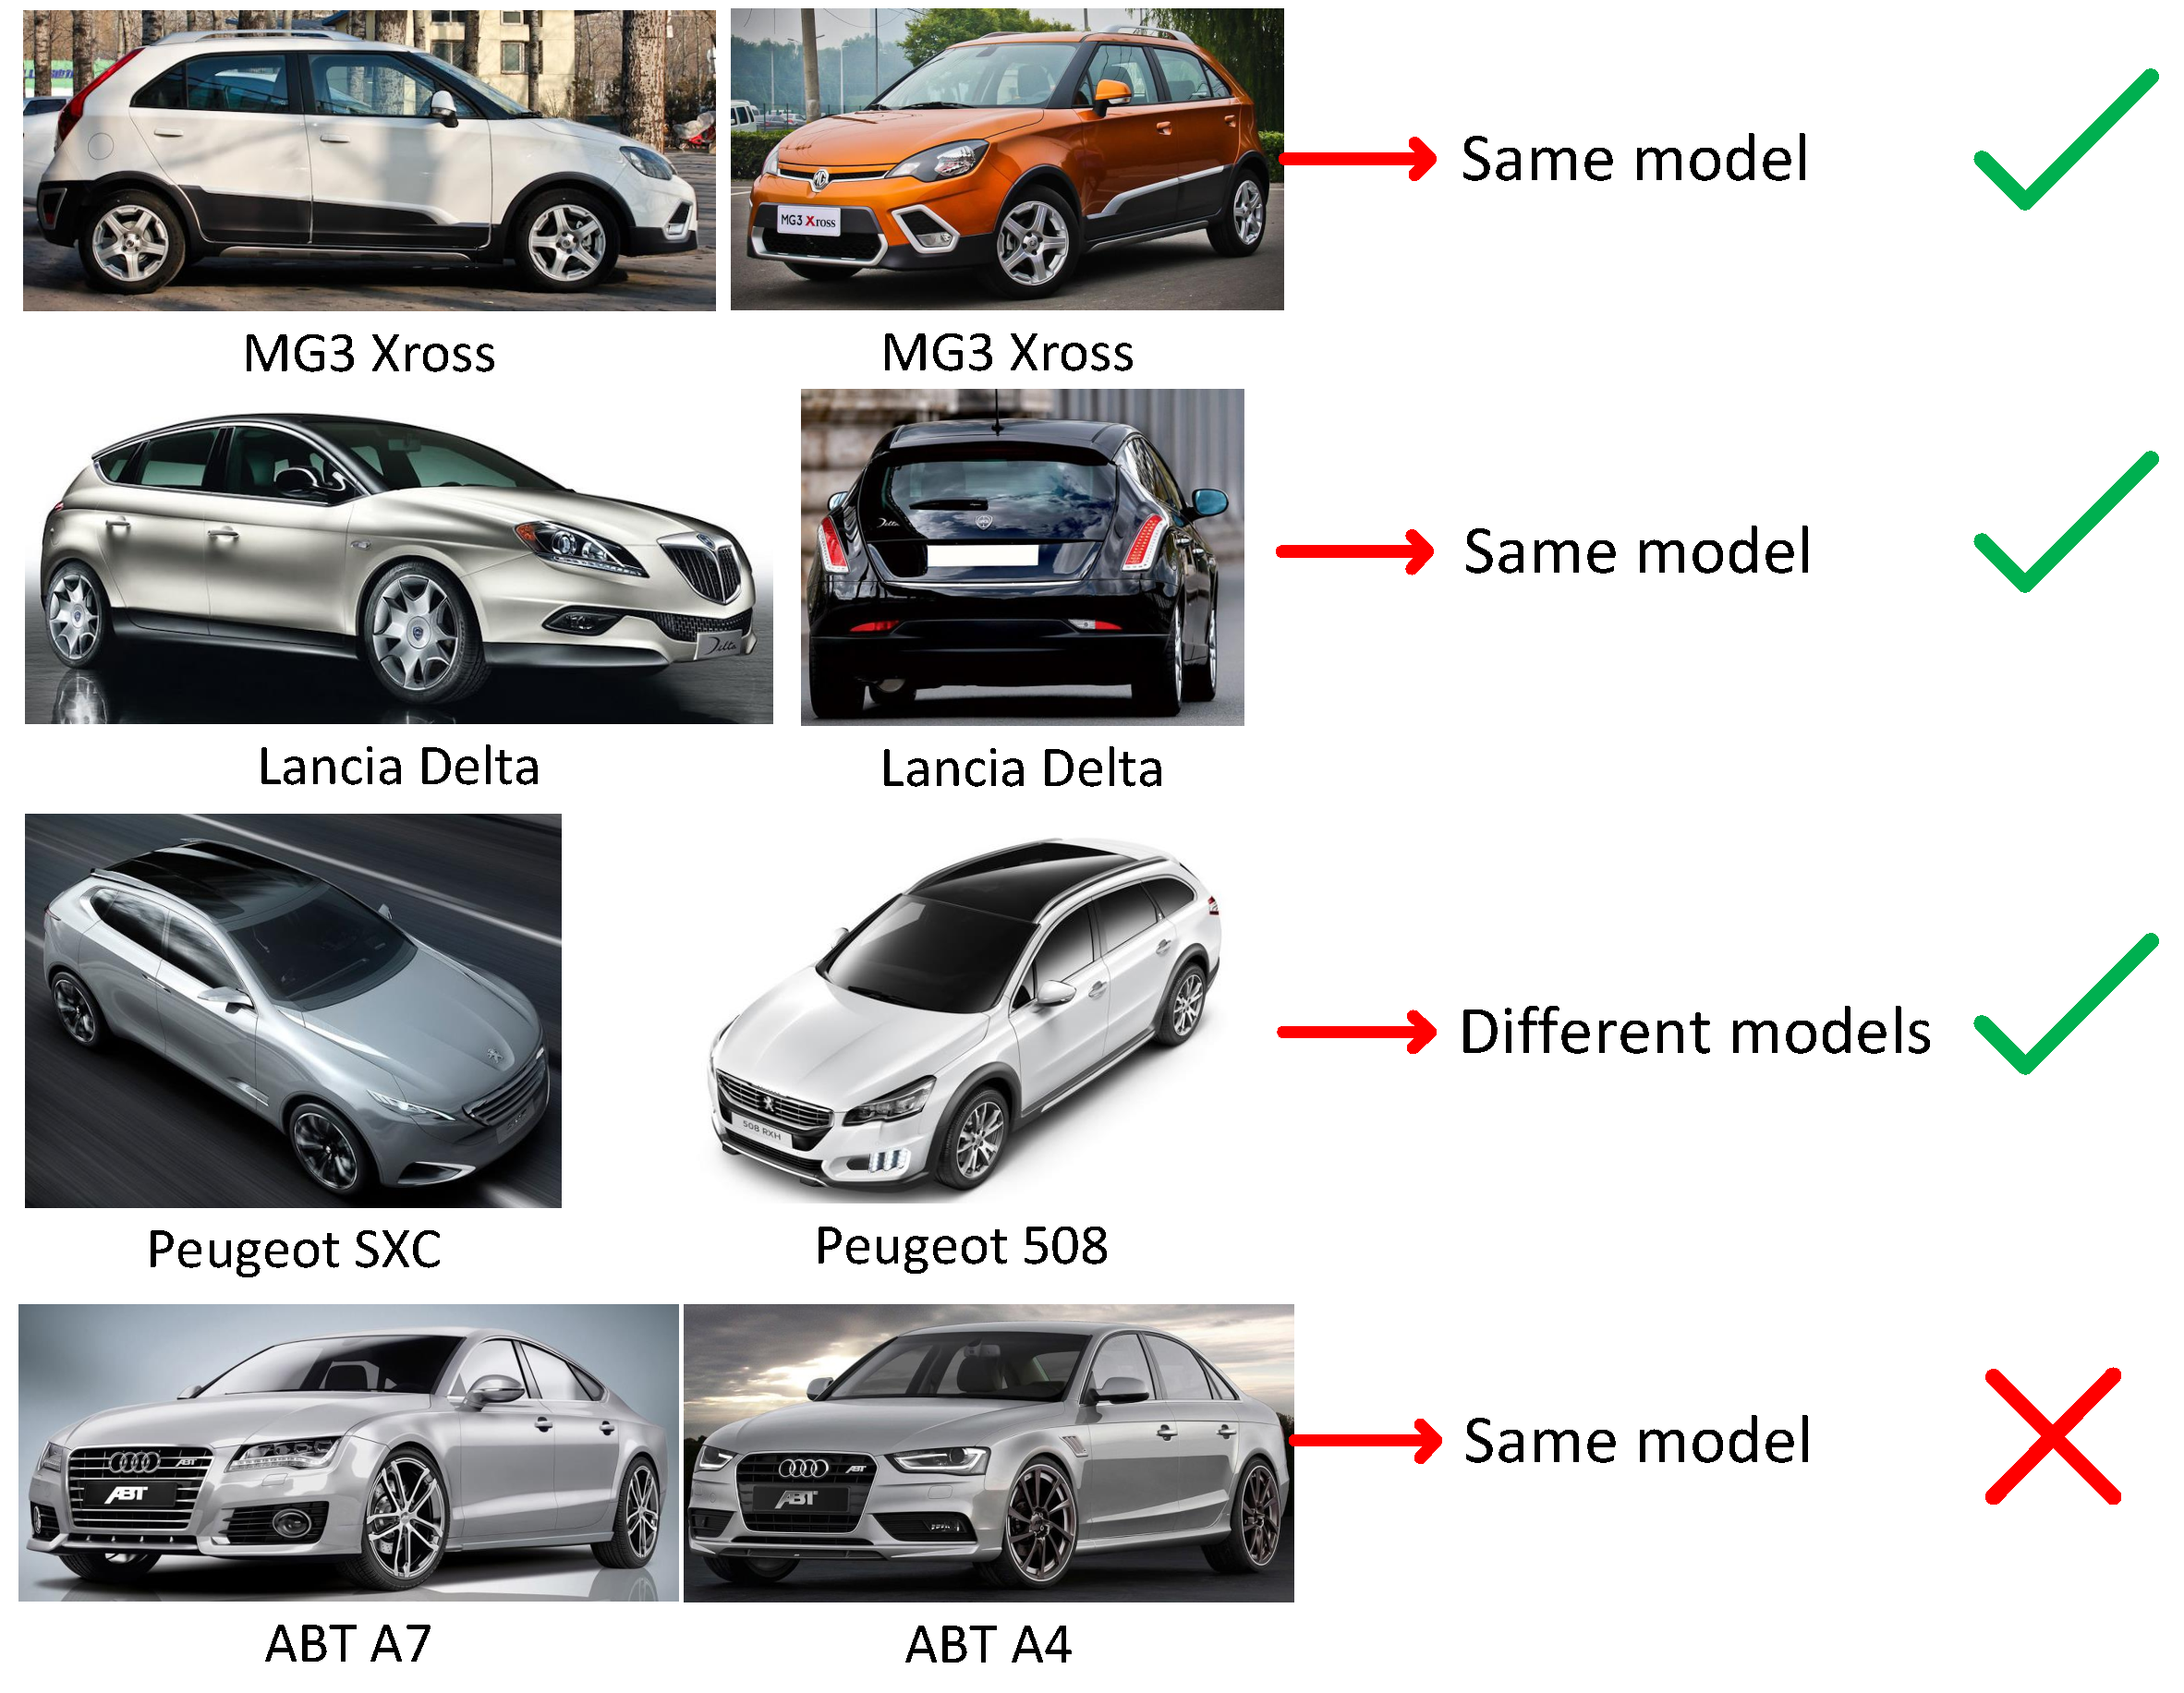
\includegraphics[width=1\linewidth]{verif.pdf}
\caption{Four test samples of verification and their prediction results. All these samples are very challenging and our model obtains correct results except for the last one. }
\label{fig:verif}
\vspace{-3pt}
\end{figure}



\begin{table}
\small
\centering
\caption{The verification accuracy of three baseline models.  }
\begin{tabular}{*{4}{|c}|}
\hline
   & Easy & Medium& Hard\\
\hline
CNN feature + Joint Bayesian  & 0.833& 0.824& 0.761 \\
\hline
CNN feature + SVM & 0.700 & 0.690 & 0.659 \\
\hline
random guess & \multicolumn{3}{c|}{0.500} \\
\hline
\end{tabular}
\label{tab:verif}
\end{table}

\begin{figure}[t]\centering
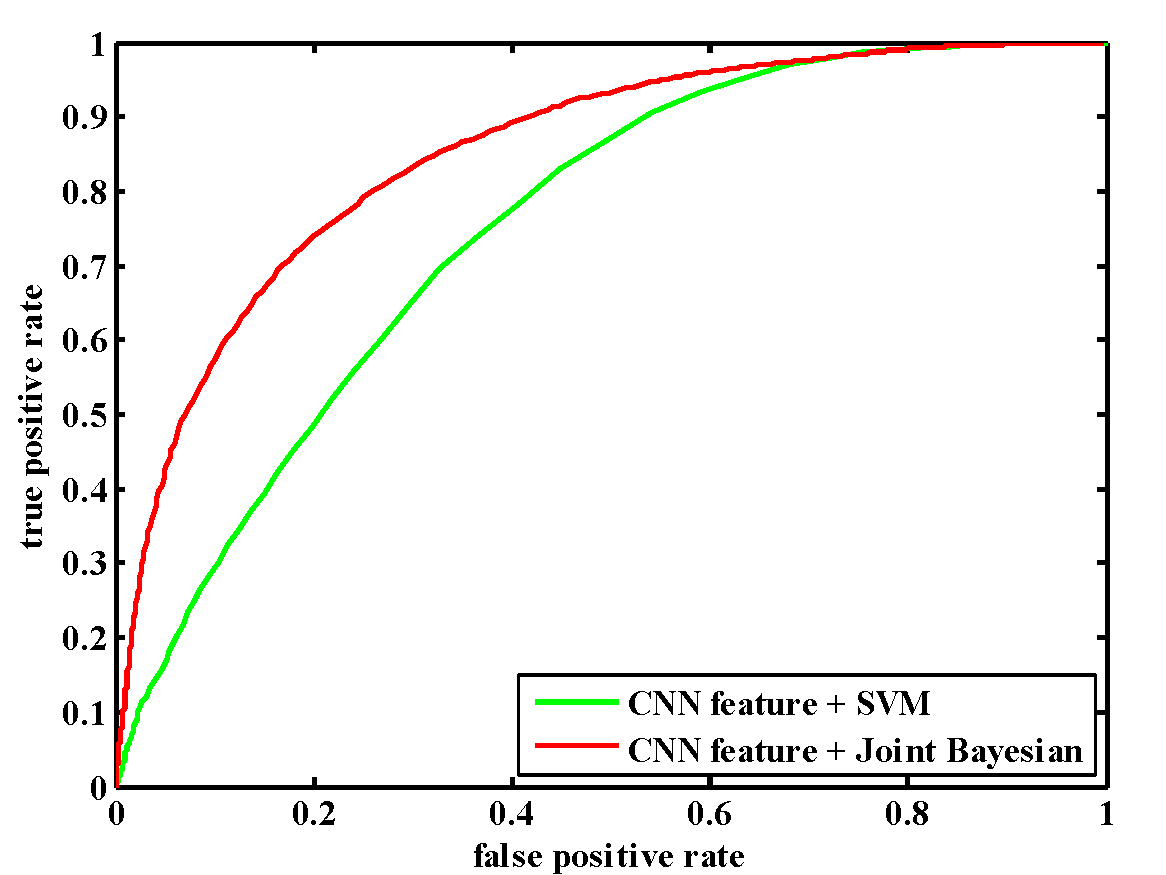
\includegraphics[width=1\linewidth]{roc.pdf}
\caption{The ROC curves of two baseline models for the hard flavor. }
\label{fig:roc}
\end{figure}

\section{Updated Results: Comparing Different Deep Models}\label{sec:updated}
As an extension to the experiments in Section~\ref{sec:exp}, we conduct experiments for fine-grained car classification, attribute prediction, and car verification with the entire dataset and different deep models, in order to explore the different capabilities of the models on these tasks. The split of the dataset into the three tasks is similar to Section~\ref{sec:exp}, where three subsets contain $431$, $111$, and $1,145$ car models, with $52,083$, $11,129$, and $72,962$ images respectively. The only difference is that we adopt full set of CompCars in order to establish updated baseline experiments and to make use of the dataset to the largest extent. We keep the testing sets of car verification same to those in Section~\ref{sec:verif}.

We evaluate three network structures, namely AlexNet~\cite{Krizhevsky12}, Overfeat~\cite{Sermanet13}, and GoogLeNet~\cite{Szegedy14} for all three tasks. All networks are pre-trained on the ImageNet classification task~\cite{Deng09}, and fine-tuned with the same mini-batch size, epochs, and learning rates for each task. All predictions of the deep models are produced with a single center crop of the image. We use Caffe~\cite{Jia14caffe} as the platform for our experiments. The experimental results can serve as baselines in any later research works. The train/test splits can be downloaded from CompCars webpage \url{http://mmlab.ie.cuhk.edu.hk/datasets/comp_cars/index.html}.

\subsection{Fine-Grained Classification}\label{sec:class}
In this section, we classify the car images into $431$ car models as in Section~\ref{sec:cls}. We divide the data into 70\% for training and 30\% for testing. We train classification models using car images in all viewpoints. The performances of the three networks are summarized in Table~\ref{tab:class}. Overfeat beats AlexNet with a large margin of 6.0\% while GoogLeNet beats Overfeat by 3.3\% in Top-1 accuracy, which is in consistency with their performances on the ImageNet classification task. Given more data, the accuracy rises about 11\% for Overfeat compared to Table~\ref{tab:cls_car}\footnote{Due to the difference in testing sets, the accuracies are not directly comparable. However a rough estimate is still viable.}. We also release the fine-tuned GoogLeNet model on the CompCars webpage.%%later to be released in the caffe model zoo

\begin{table}
\small
\centering
\caption{The classification accuracies of three deep models.}
\begin{tabular}{*{4}{|c}|}
\hline
Model & AlexNet  & Overfeat & GoogLeNet \\
\hline
Top-1 & 0.819 &	0.879 & 0.912 \\
 \hline
Top-5 & 0.940 & 0.969 & 0.981 \\
 \hline

\end{tabular}
\label{tab:class}
\end{table}

\subsection{Attribute Prediction}\label{sec:attr_up}
We predict attributes from $111$ models not existed in the training set. Different from Section~\ref{sec:attr} where models are trained with cars in single viewpoints, we train with images in all viewpoints to build a compact model. Table~\ref{tab:attr_up} summarizes the results for the three networks, where ``mean guess'' represents the prediction with the mean of the values on the training set. GoogLeNet performs the best for all attributes and Overfeat is a close running-up.

\begin{table}
\small
\centering
\caption{Attribute prediction results of three deep models. For the continuous attributes (maximum speed and displacement), we display the mean difference from the ground truth (lower is better). For the discrete attributes (door and seat number, car type), we display the classification accuracy (higher is better).}
\begin{tabular}{*{4}{|c}|}
\hline
Model & AlexNet  & Overfeat & GoogLeNet \\
\hline
& \multicolumn{3}{c|}{mean difference} \\
\hline
Maximum speed & 21.3 &	19.4 & 19.4  \\
\cline{2-4}
(mean guess) &\multicolumn{3}{c|}{36.9 } \\
\cline{2-4}
Displacement & 0.803 & 0.770 & 0.760  \\
\cline{2-4}
(mean guess) &\multicolumn{3}{c|}{1.02 } \\
 \hline
& \multicolumn{3}{c|}{classification accuracy} \\
\hline
Door number & 0.750 &0.780 & 0.796 \\
Seat number & 0.691&0.713 &0.717  \\
Car type & 0.602& 0.631 & 0.643 \\
\hline
\end{tabular}
\label{tab:attr_up}
\end{table}

\subsection{Car Verification}
The evaluation pipeline follows Section~\ref{sec:verif}. We evaluate the three deep models combined with two verification models: Joint Bayesian~\cite{Chen12} and SVM with polynomial kernel. The feature extracted from the CNN models is reduced to $200$ by PCA before training and testing in all experiments.

The performances of the three networks combined with the two verification models are shown in Table~\ref{tab:verif_up}, where each model is denoted by \{name of the deep model\} + \{name of the verification model\}. GoogLeNet + Joint Bayesian achieves the best performance in all three settings. For each deep model, Joint Bayesian outperforms SVM consistently. Compared to Table~\ref{tab:verif}, Overfeat + Joint Bayesian yields a performance gain of $2\sim4\%$ in the three settings, which is purely due to the increase in training data.
The ROC curves for the three sets are plotted in Figure~\ref{fig:roc}.

\begin{table}
\small
\centering
\caption{The verification accuracies of six models.}
\begin{tabular}{*{4}{|c}|}
\hline
  & Easy  & Medium & Hard \\
\hline
AlexNet + SVM & 0.822 &	0.800 & 0.729 \\
 \hline
AlexNet + Joint Bayesian & 0.853 &	0.823 & 0.774 \\
 \hline
Overfeat + SVM & 0.860 & 0.830 & 0.754 \\
 \hline
Overfeat + Joint Bayesian & 0.873 &	0.841 & 0.780 \\
 \hline
GoogLeNet + SVM & 0.880 &	0.837 & 0.764 \\
 \hline
GoogLeNet + Joint Bayesian & 0.907 & 0.852 & 0.788 \\
 \hline
\end{tabular}
\label{tab:verif_up}
\end{table}

\begin{figure}[t]
\small\centering
\begin{minipage}[t]{0.9\linewidth}
\centering
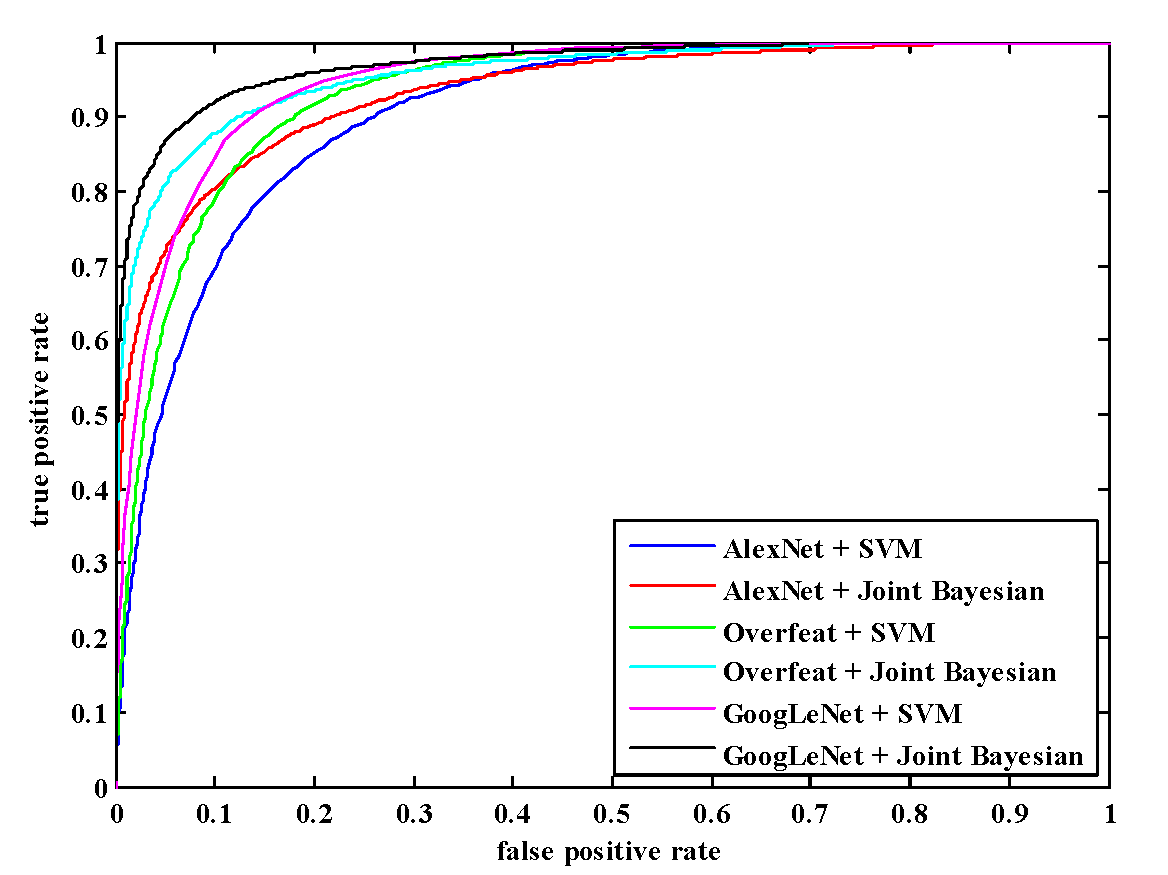
\includegraphics[height=2.2in]{roc1.pdf}
\par{(a)}
\end{minipage}
\begin{minipage}[t]{0.9\linewidth}
\centering
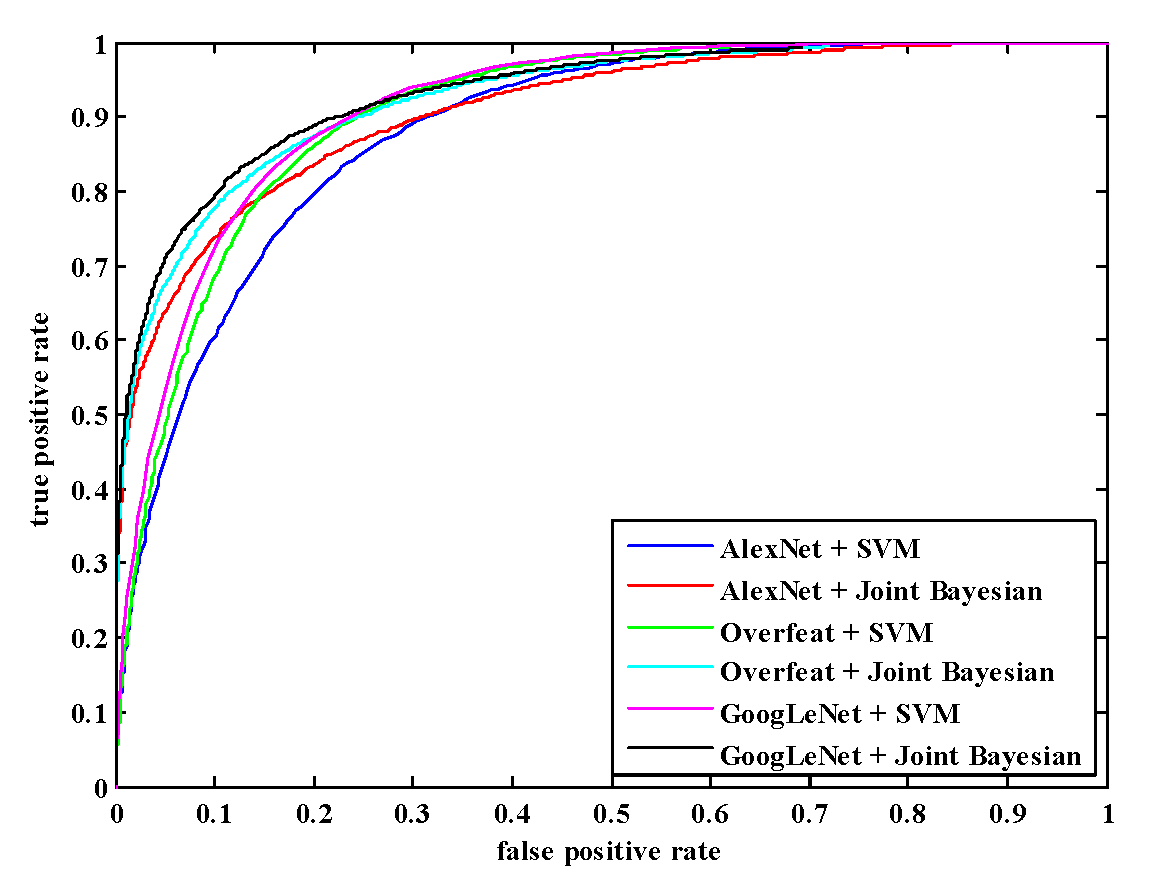
\includegraphics[height=2.2in]{roc2.pdf}
\par{(b)}
\end{minipage}
\begin{minipage}[t]{0.9\linewidth}
\centering
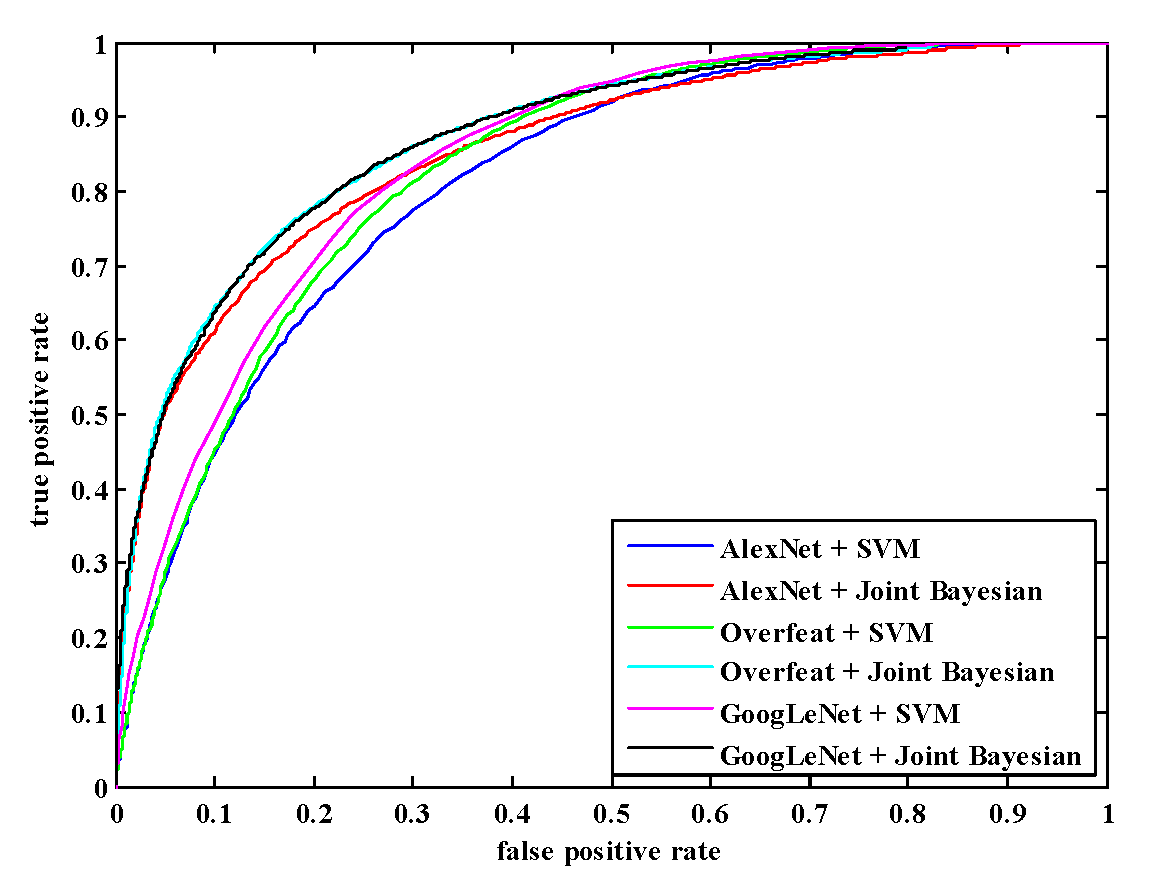
\includegraphics[height=2.2in]{roc3.pdf}
\par{(c)}
\end{minipage}
\caption{The ROC curves of six verification models for (a) easy, (b) medium, and (c) hard set. }
\label{fig:roc}
\end{figure}

\section{Fine-Grained Classification with Surveillance Data}\label{sec:surveillance}
This is a follow-up experiment for fine-grained classification with surveillance-nature data. The data includes $44,481$ images in $281$ different car models. 70\% images are for training and 30\% are for testing. The car images are all in front views with various environment conditions such as rainy, foggy, and at night. We adopt the same three network structures (AlexNet, Overfeat, and GoogLeNet) as in the web-nature data applications for this task. The networks are also pre-trained on the ImageNet classification task, and the test is done with a single center crop. The car images are first cropped with the labeled bounding boxes with paddings of around 7\% on each side. All cropped images are resized to $256\times256$ pixels. The experimental results are shown in Table~\ref{tab:surveillance}. The three networks all achieve very high accuracies for this task. The result indicates that the fixed view (front view) greatly simplifies the fine-grained classification task, even when large environmental differences exist.

\begin{table}
\small
\centering
\caption{The classification accuracies of three deep models on surveillance data.}
\begin{tabular}{*{4}{|c}|}
\hline
Model & AlexNet  & Overfeat & GoogLeNet \\
\hline
Top-1 & 0.980 &	0.983 & 0.984 \\
 \hline
\end{tabular}
\label{tab:surveillance}
\end{table}

\section{Discussions}\label{sec:discussion}

In this paper, we wish to promote the field of research related to ``cars'', which is largely neglected by the computer vision community. To this end, we have introduced a large-scale car dataset called \datasetName{}, which contains images with not only different viewpoints, but also car parts and rich attributes. \datasetName{} provides a number of unique properties that other fine-grained datasets do not have, such as a much larger subcategory quantity, a unique hierarchical structure, implicit and explicit attributes, and large amount of car part images which can be utilized for style analysis and part recognition. It also bears cross modality nature, consisting of web-nature data and surveillance-nature data, ready to be used for cross modality research.
%
To validate the usefulness of the dataset and inspire the community for other novel tasks, we have conducted baseline experiments on three tasks: car model classification, car model verification, and attribute prediction. The experimental results reveal several challenges of these tasks and provide qualitative observations of the data, which is beneficial for future research.

There are many other potential tasks that can exploit \datasetName{}. Image ranking is one of the long-lasting topics in the literature, car model ranking can be adapted from this line of research to find the models that users are mostly interested in. The rich attributes of the dataset can be used to learn the relationships between different car models. Combining with the provided 3-level hierarchy, it will yield a stronger and more meaningful relationship graph for car models. Car images from different viewpoints can be utilized for ultra-wide baseline matching and 3D reconstruction, which can benefit recognition and verification in return.
%Any other interesting tasks? You name it.
%%We believe this new dataset will inspire the community for a range of novel vision tasks and promote the development of computer vision.



{\small
\bibliographystyle{ieee}
\bibliography{egbib}
}

\end{document}
